\documentclass[journal,twoside,web]{ieeecolor}
\usepackage{generic}
\usepackage{amsmath,amssymb,amsfonts,bm}
\usepackage{graphicx}
\usepackage{rotating}
% \usepackage{subfigure}
\usepackage[format=default,justification=centerlast]{caption} % Figure caption text customization 

\usepackage[list=true,labelformat=simple]{subcaption}
\renewcommand\thesubfigure{(\alph{subfigure})}
\graphicspath{%
  {figs/matlab/}
} 

\usepackage{pgfgantt}

\usepackage{booktabs,array} % Packages for tables

\usepackage{hyperref}
\usepackage[colorinlistoftodos]{todonotes}
\usepackage{soul}
\usepackage{easyReview}
\usepackage{setspace}
\usepackage{multirow}

\usepackage[ruled, vlined, linesnumbered]{algorithm2e} % For algorithms

\usepackage{tikz}
\usetikzlibrary{shapes,arrows, positioning, quotes}
\usetikzlibrary{arrows.meta, positioning, decorations.markings}
\usetikzlibrary{calc,tikzmark}
\usetikzlibrary{backgrounds,calc,patterns,decorations.pathmorphing,decorations.markings,shapes,arrows,snakes,tikzmark}

\usepackage{siunitx}
% \sisetup{unitsep=\cdot}
% \usepackage{textcomp}
\def\BibTeX{{\rm B\kern-.05em{\sc i\kern-.025em b}\kern-.08em
    T\kern-.1667em\lower.7ex\hbox{E}\kern-.125emX}}
\markboth{\journalname, VOL. XX, NO. XX, XXXX}
{Author \MakeLowercase{\textit{et al.}}: Title}
\begin{document}
\title{Hardware-in-the-Loop Plant Modeling for Autonomous Vehicle}
\author{First A. Author, \IEEEmembership{Fellow, IEEE}, Second B. Author, and Third C. Author, Jr., \IEEEmembership{Member, IEEE}
\thanks{This paragraph of the first footnote will contain the date on 
which you submitted your paper for review. It will also contain support 
information, including sponsor and financial support acknowledgment. For 
example, ``This work was supported in part by the U.S. Department of 
Commerce under Grant BS123456.'' }
\thanks{The next few paragraphs should contain 
the authors' current affiliations, including current address and e-mail. For 
example, F. A. Author is with the National Institute of Standards and 
Technology, Boulder, CO 80305 USA (e-mail: author@boulder.nist.gov). }
\thanks{S. B. Author, Jr., was with Rice University, Houston, TX 77005 USA. He is 
now with the Department of Physics, Colorado State University, Fort Collins, 
CO 80523 USA (e-mail: author@lamar.colostate.edu).}
\thanks{T. C. Author is with 
the Electrical Engineering Department, University of Colorado, Boulder, CO 
80309 USA, on leave from the National Research Institute for Metals, 
Tsukuba, Japan (e-mail: author@nrim.go.jp).}
}

\maketitle

\begin{abstract}
This report presents the results of modeling vehicle systems and testing them using Hardware-in-the-Loop (HIL). First, data was collected for each system using a Lexus RX450H vehicle. After data collection, models were developed in order to accurately simulate the physical vehicle system. MATLAB’s System Identification Toolbox was initially used to create these models. However, the transfer function models it provided weren’t able to accurately represent these systems and their non-linear behaviors. After this was established, modeling was done using MATLAB’s Neural Network Time Series application. Once a Neural Network model was created, it was then exported to Simulink and modified to be able to run without the use of the Deep Learning toolbox. These models gave much more accurate results when compared to the transfer function models developed using the System Identification Toolbox. (Add section about testing and results). 

%These instructions give you guidelines for preparing papers for 
%IEEE Transactions and Journals. Use this document as a template if you are 
%using \LaTeX. Otherwise, use this document as an 
%instruction set. The electronic file of your paper will be formatted further 
%at IEEE. Paper titles should be written in uppercase and lowercase letters, 
%not all uppercase. Avoid writing long formulas with subscripts in the title; 
%short formulas that identify the elements are fine (e.g., "Nd--Fe--B"). Do 
%not write ``(Invited)'' in the title. Full names of authors are preferred in 
%the author field, but are not required. Put a space between authors' 
%initials. The abstract must be a concise yet comprehensive reflection of 
%what is in your article. In particular, the abstract must be self-contained, 
%without abbreviations, footnotes, or references. It should be a microcosm of 
%the full article. The abstract must be between 150--250 words. Be sure that 
%you adhere to these limits; otherwise, you will need to edit your abstract 
%accordingly. The abstract must be written as one paragraph, and should not 
%contain displayed mathematical equations or tabular material. The abstract 
%should include three or four different keywords or phrases, as this will 
%help readers to find it. It is important to avoid over-repetition of such 
%phrases as this can result in a page being rejected by search engines. 
%Ensure that your abstract reads well and is grammatically correct.
\end{abstract}

\begin{IEEEkeywords}
Hardware-in-the-Loop, Neural Network, System Identification
\end{IEEEkeywords}

\section{Introduction}
\label{sec:introduction}
\IEEEPARstart{A}{utonomous} vehicles are being developed by many companies for commercial and
personal use. These autonomous vehicles (see the AutonomouStuff vehicle fleet
shown in Fig.~\ref{fig:fleet}) would allow companies to continue crucial deliveries
or transports of their products even if there is a shortage of drivers. In
addition, autonomous vehicles have the ability to make roads safer for drivers
and pedestrians alike. To develop a reliable and safe transportation system for
modern world, a large body of research in the field of autonomous vehicles is
being conducted in recent decades \cite{Liu2017} \cite{Prasad2020}.
Therefore, it is apparent that researchers of the autonomous vehicle community
have been focusing on analysis, design, and development of different subsystems
of self-driving/autonomous vehicles. Furthermore, modeling vehicle subsystems is
a pre-requisite for the development of reliable controllers for these vehicles
to be managed in the era of modern transportation systems in general.

% \vspace*{12pt}

\noindent Usually, there are six main subsystems of a self-driving vehicle: %
%
\begin{enumerate}
\item  Steering,
  
\item acceleration,
  
\item brake,
  
\item shift,

\item speed, and 
  
\item speed control (cruise) subsystems.
\end{enumerate}
%
These subsystems are to be modeled to get an accurate representation of how
the vehicle should be controlled. Within the scope of this project and to expedite the modeling process, commercially available modeling tools in Mathworks' MATLAB, System Identification app in the System Identification Toolbox and Neural Network Time Series app in the Deep Learning toolbox, were used to model six subsystems for a Lexus vehicle platform, which is an experimental autonomous vehicle platform that belongs to AutonomouStuff Solutions~\footnote{\url{https://autonomoustuff.com/}}. The first subsystem we will model is the steering model, and then we will move onto
the other subsystems. There are already controllers in place for the Lexus
vehicle platform, but their reliability is lower than expected due to non-linear
behaviors of the torque voltages required to control each subsystem. The scope
of this project includes developing mathematical models for each subsystem so
AutonomouStuff can implement control systems that improve the reliability of the
autonomous vehicle platform. These models will be considered reliable if they can track actual vehicle subsystem behaviors with a minimum best fit percentage between 85 to 95 percent and fall within the error bounds defined for each subsystem. Once these models are developed, they will be tested using AutonomouStuff's Hardware-in-the-Loop (HIL) bench.
Once there is confidence in each model, AutonomouStuff can use these models on their HIL bench to develop controllers that will remove the non-linear behaviors of each vehicle subsystem.
There are two operating modes of the Lexus vehicle platform used in this project: Manual-drive and by-wire or autonomous.
Fig.~\ref{fig:steerOverview} depicts how the by-wire mode controls the vehicle. Each
subsystem, like the steering system in this example, sends torque voltages to a
motor that will control the subsystem. In Fig.~\ref{fig:steerOverview}, the motor would
turn the pinion arms which would change the steering angle of the vehicle. This
principle is applied to all other subsystems.

\vspace*{12pt}

\begin{figure}[htbp]
  \centering
  \begin{subfigure}[b]{0.48\linewidth}
    \centering
    \includegraphics[height=3cm]{figs/img/autonomousVehiclesAStuff}
    \caption{}
    \label{fig:fleet}
  \end{subfigure}
  \begin{subfigure}[b]{0.48\linewidth}
    \centering
    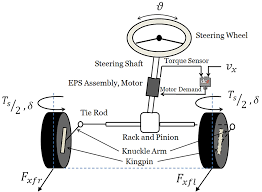
\includegraphics[height=3cm]{figs/img/autonomousVehiclesSteering}
    \caption{}
    \label{fig:steerOverview}
  \end{subfigure}
  \caption{\subref{fig:fleet} Autonomous vehicle fleet in AutonomouStuff Solutions and \subref{fig:steerOverview} steering model setup (courtesy of AutonomouStuff). }
  \label{fig:AstuffFleetSteeringSetup}
\end{figure}


 \section{Literature Review}

 Authors in~\cite{Hussain2011} illustrates identification of multiple-input
 single-output model for maximum power point tracking of photovoltaic system. A
 significant effort was conducted to model the photovoltaic system, where the two inputs were
 Solar irradiance and Cell temperature, and the output was DC current. To model
 this system, Matlab’s System Identification Toolbox was used. In order to
 create different models, they collected and used data from an energy center in
 Malaysia. After generating different models, the authors ended up going with a
 fourth order ARX (also known as ARXQS) model because it was the most accurate,
 with a best fit percentage of 93.42\%. The polynomial model equation for ARX is
 shown below. %
 %
 \begin{multline*}
   y(t) + a_1y(t - 1) +...+a_{na}y(t - n_{a}) = \\
   b_{1}u_{1}(t-n_{k})+...+b_{nb}u_{nb}(t - n_{k}-n_{b}+1) + e(t), 
 \end{multline*}
% 
$y(t)$ is the system output at time $t,$ while $u(t)$ is the input. The noise disturbance of the system is represented by $e(t).$ The variables $na,$ $nb,$ and $nk$ are the system’s number of poles, amount of $b$ parameters, and the samples before the inputs begin to affect the system’s output.



\section{System Identification Preliminaries}

System identification is the process of developing mathematical models for a dynamic system using the measurement of input and output signals of that system. There are many components that are used to accomplish a task that they are assigned without knowing the exact behavior of the system for given input signals. Without knowing the response of this black-box, there could be unexpected consequences from a system. The goal of the system identification methodology is to get an accurate estimation of the system response to any given input. Mathworks' MATLAB has the System Identification Toolbox, where a few existing examples demonstrate the working principle of this toolbox.

\subsection{Example 1: Dealing with Multi-Variable Systems: Identification and Analysis}
\label{sec:sysID-Example1}

The example given in~\cite{example1} shows how to create an iddata object from a
dataset in order to get the inputs and the outputs. The next step was to look at
the impulse and step responses in order to learn more about how the inputs and
outputs act. From there the state space model was estimated using the first part
of the given data. This model was compared to the step responses and with the
second part of the data to see if it was a good fit. The model had a best fit
percentage of 83.55\% for the generated voltage data, and a best fit of 39.33\%

for the speed data. The frequency response of the model was estimated with
spectral analysis and bode plots were also created. The tutorial explained that
if the data doesn’t give nice models, then it is best to try out submodels for
the different channels. Two single-input single-output (SISO) models were
created and compared with the existing multiple-input multiple-output (MIMO)
model and the actual data. The Nyquist plots were also compared. Both SISO
models performed well during these comparisons. The next step in the tutorial
was to create a multiple-input single-output (MISO) model in order to get a
model that more accurately reflected the generated voltage data. By creating
this model and comparing it to the validation data and previous models, we saw a
best fit percentage of 90.18\%. The last thing the example showed was how to
merge the two SISO models we created earlier.

\begin{figure}[htbp]
    \centering
    % \captionsetup{justification=centering, margin=3cm}
    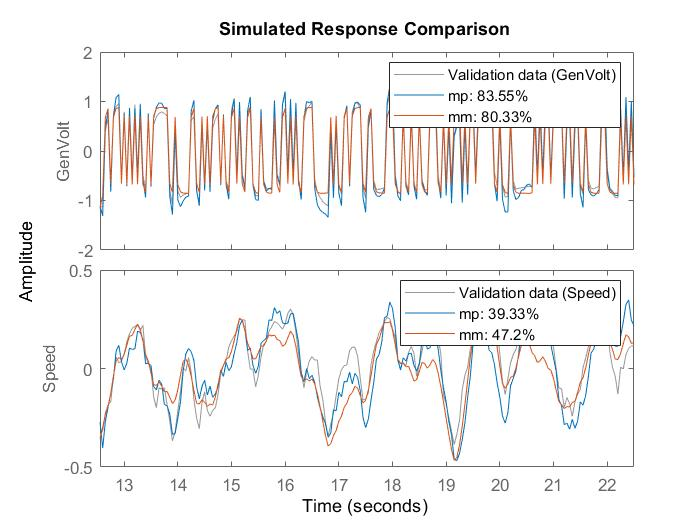
\includegraphics[width=2.5in]{figs/img/mimoExGrady}
    \caption{Comparison of the state space model and merged SISO models with the validation data}
    \label{fig:exMIMO}
\end{figure}

\subsection{Example 2: Selecting Model Structures for Multivariable Systems}
\label{sec:sysID-Example2}
This example~\cite{Matlab2} discusses solutions for modeling both MISO and MIMO models using Mathworks' Matlab System Identification Toolbox. As the article discusses, MISO system models are easier to develop because all model structures used by the toolbox support models with a single output and multiple inputs. Therefore, the process for developing a model for a MISO system is importing the data as an iddata object, removing the mean from the data, and estimating the solution using any model structure available in the toolbox. The command line can be used by using the function associated with the model structure name and then using the compare function to get the best fit percentage. For MIMO systems, there are not model structures built into the System Identification Toolbox and they must be imported instead. Otherwise the process is very similar to that of a MISO system. For a MIMO system, using the compare function can be crucial. The compare function will tell which output channel is the most difficult to develop a model for, if it is possible at all. With this information, the output channel that is hardest to model should first be modeled individually because there will be less freedom in what model structures are available. The other channels should be able to closely relate to the model for the output channel you selected.

\begin{figure}[htbp]
  \centering
  \begin{subfigure}[b]{\linewidth}
    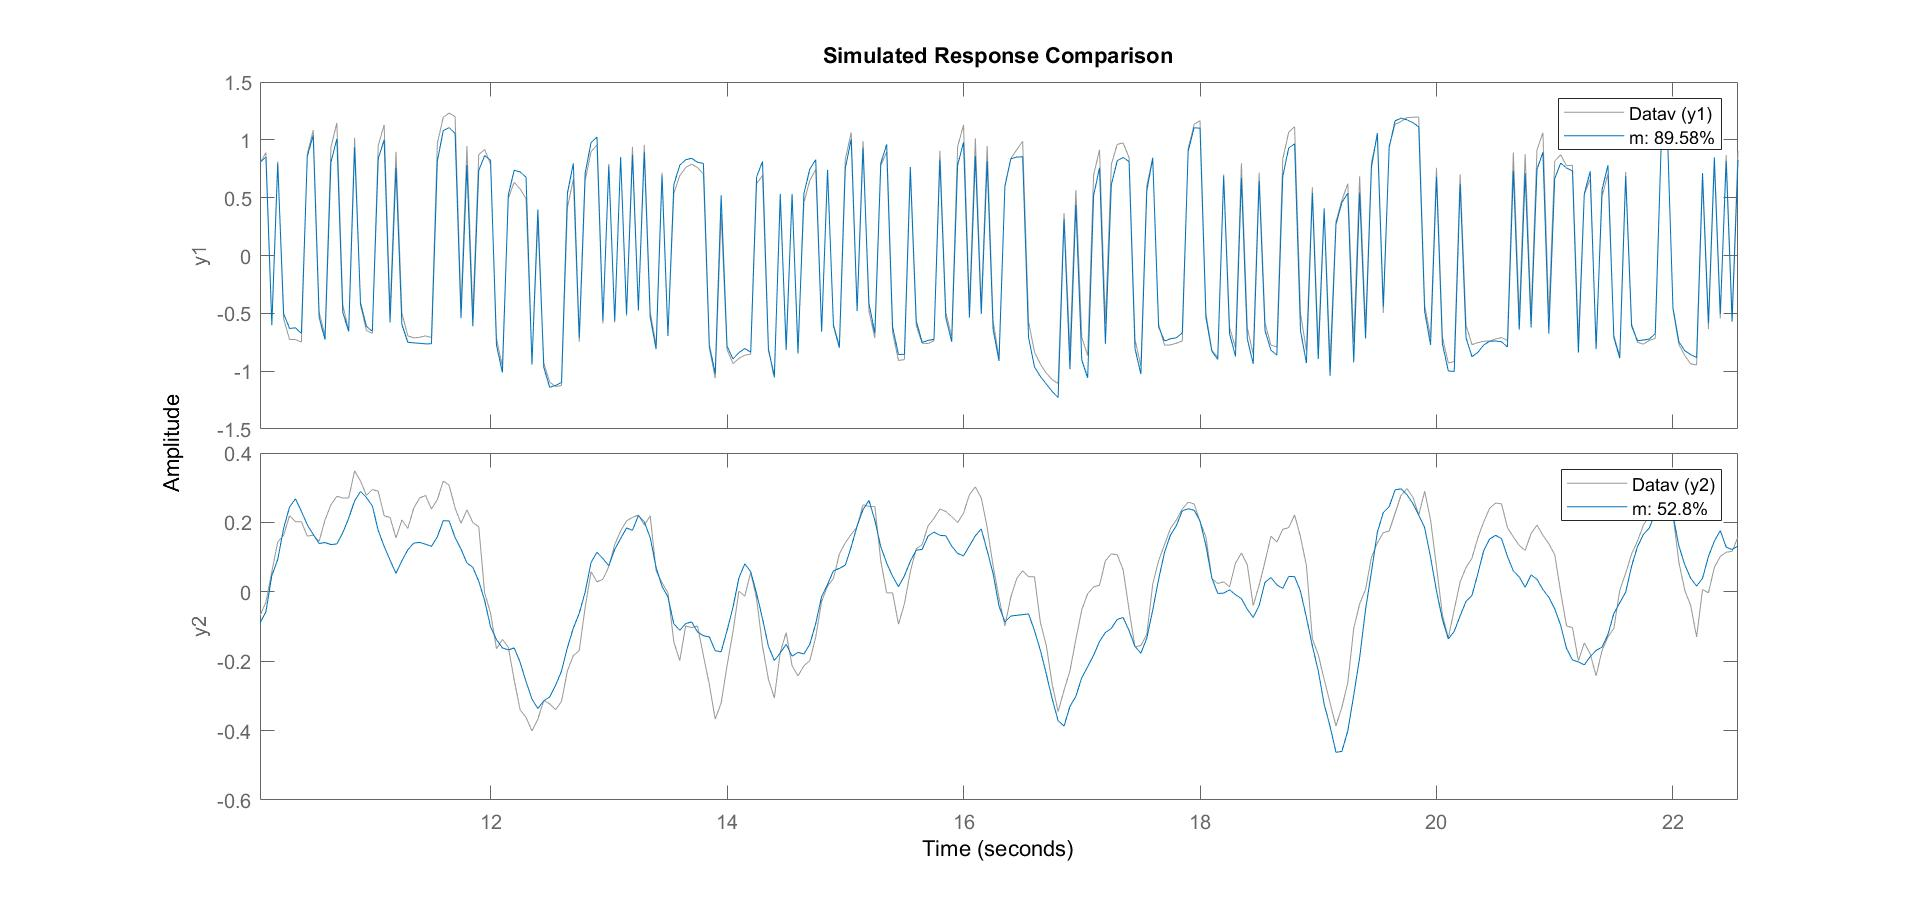
\includegraphics[height=4.25cm]{figs/img/example2Fig1}
    \caption{}
    \label{fig:ex2fig1}
  \end{subfigure}
  \\
  \begin{subfigure}[b]{\linewidth}
    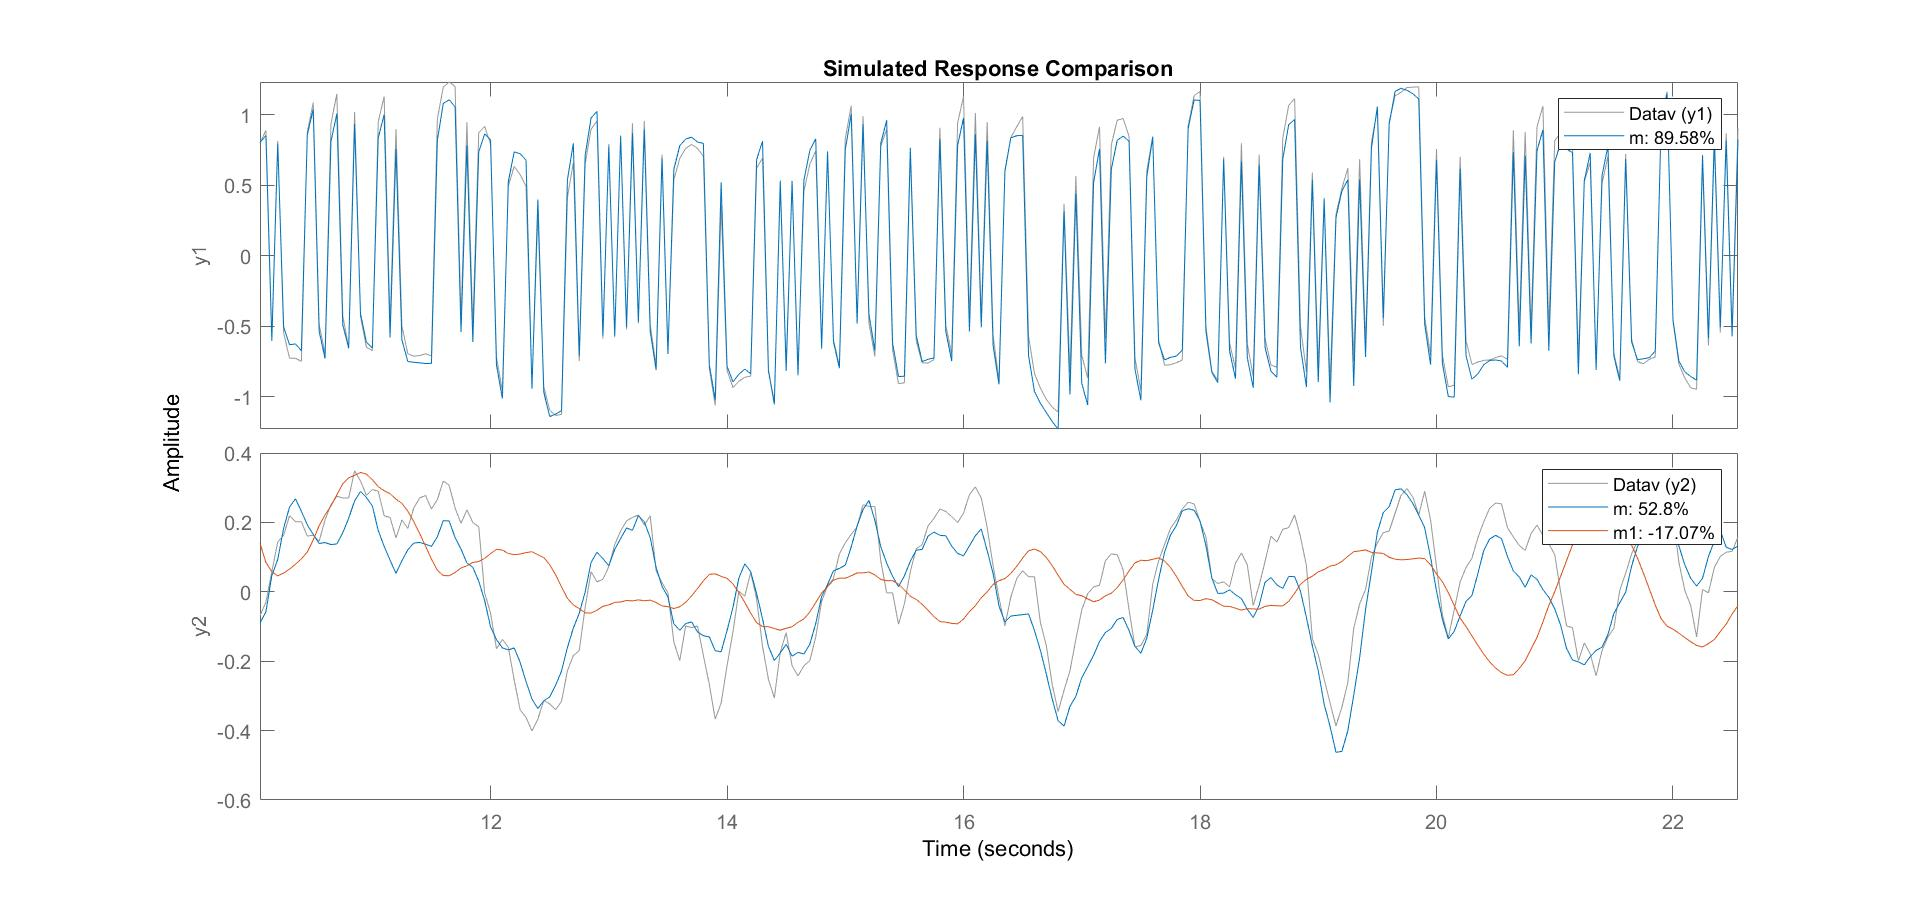
\includegraphics[height=4.25cm]{figs/img/example2Fig2}
    \caption{}
    \label{fig:ex2fig2}
  \end{subfigure}
  \caption{\subref{fig:ex2fig1} State-space model of a MIMO system with a validation data comparison and \subref{fig:ex2fig2} State-space model of a MIMO system and system-sized based state-space model with a validation data comparison }
  \label{fig:ex2}
\end{figure}

\subsection{Example 3: Identify Linear Models Using the Command Line}
\label{sec:sysID-Example3}
This example in~\cite{example3} shows how to create models for MISO systems
using the command line. Before starting the model estimation process, the
equilibrium values of the inputs and outputs had to be taken out. The data from
each experiment also had to be separated into different iddata objects. The
example showed how to estimate and compare non-parametric impulse response,
transfer function, ARMA, state-space, and Box-Jenkins models with the measured
experimental data. The state-space model with the five-step response prediction
was the most accurate, with a best fit percentage of 85.83\%.
\begin{figure}[htbp]
    \centering
    % \captionsetup{justification=centering, margin=3cm}
    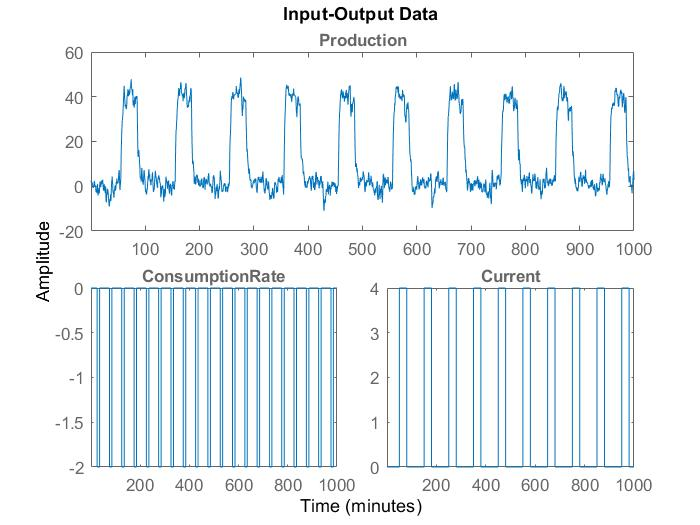
\includegraphics[width=2.5in]{figs/img/commandLineIO}
    \caption{Inputs and outputs of the given system}
    \label{fig:exIO}
\end{figure}


\section{System Architecture}
The overall system architecture of this project consists of six subsystems which are the steering, acceleration, brake, speed, shift, and speed control systems. Each of the six subsystems will be treated as a multiple-input single-output (MISO) system. For each subsystem, every input that is a torque voltage is actually two torque voltage signals, and thus can not be treated as a single input. Also, each subsystem will be treated as a single output system. The brake subsystem is shown to have two outputs but the behaviors of one of the outputs is already known so it will be modeled based on the other output's behavior. 
%
\begin{figure}[htbp]
  \centering
  %  \missingfigure{Place a high level block diagram including picture of Lexus vehicle that we are modeling}
  	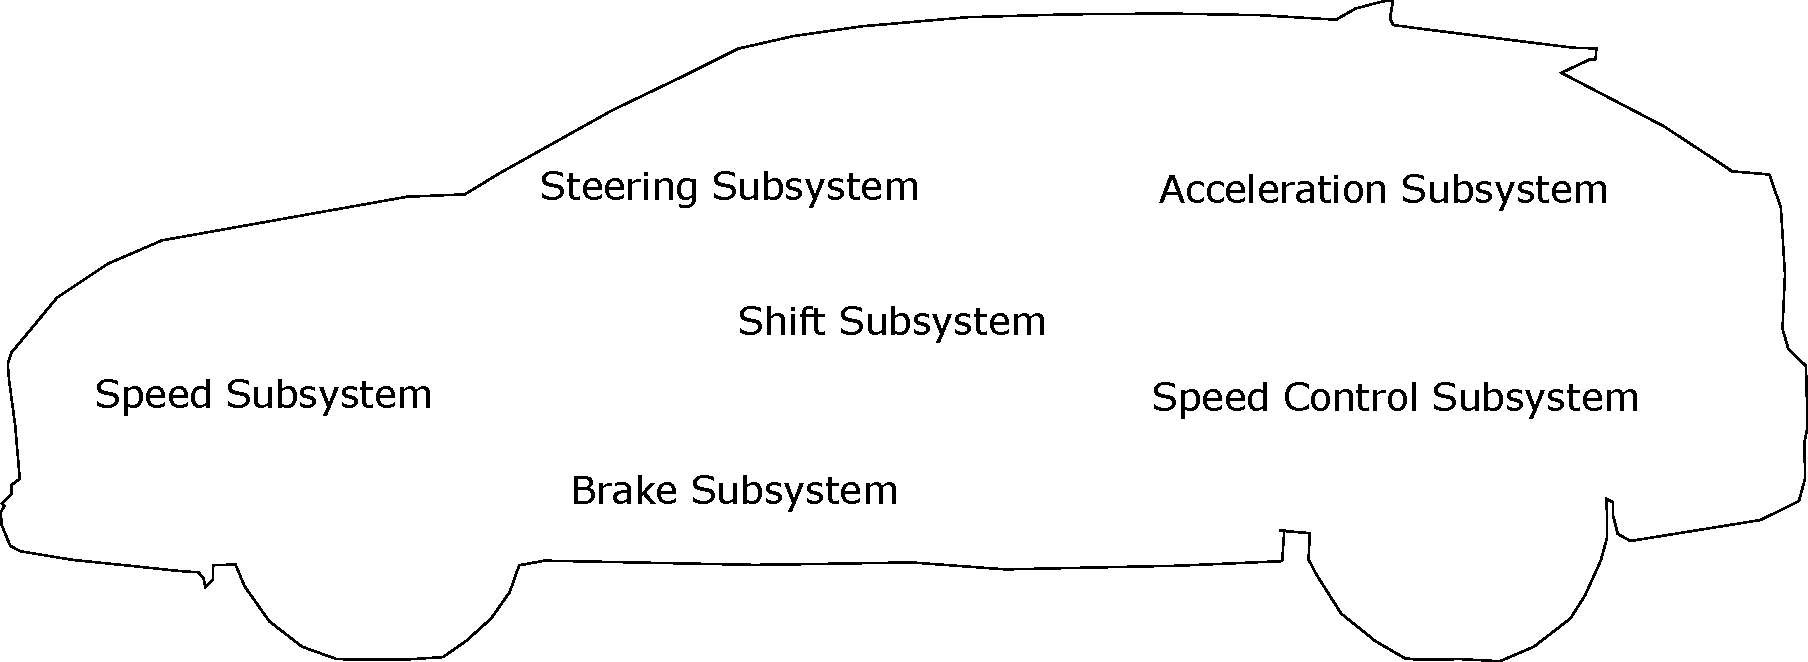
\includegraphics[height=3cm]{figs/inkscape/carSystemModelOutline}
  \caption{Hexagon Lexus self-driving vehicle showing different subsystems}
  \label{fig:highLevelSystemArchitecture}
\end{figure}

% 
\begin{figure}[htbp]
	\centering
	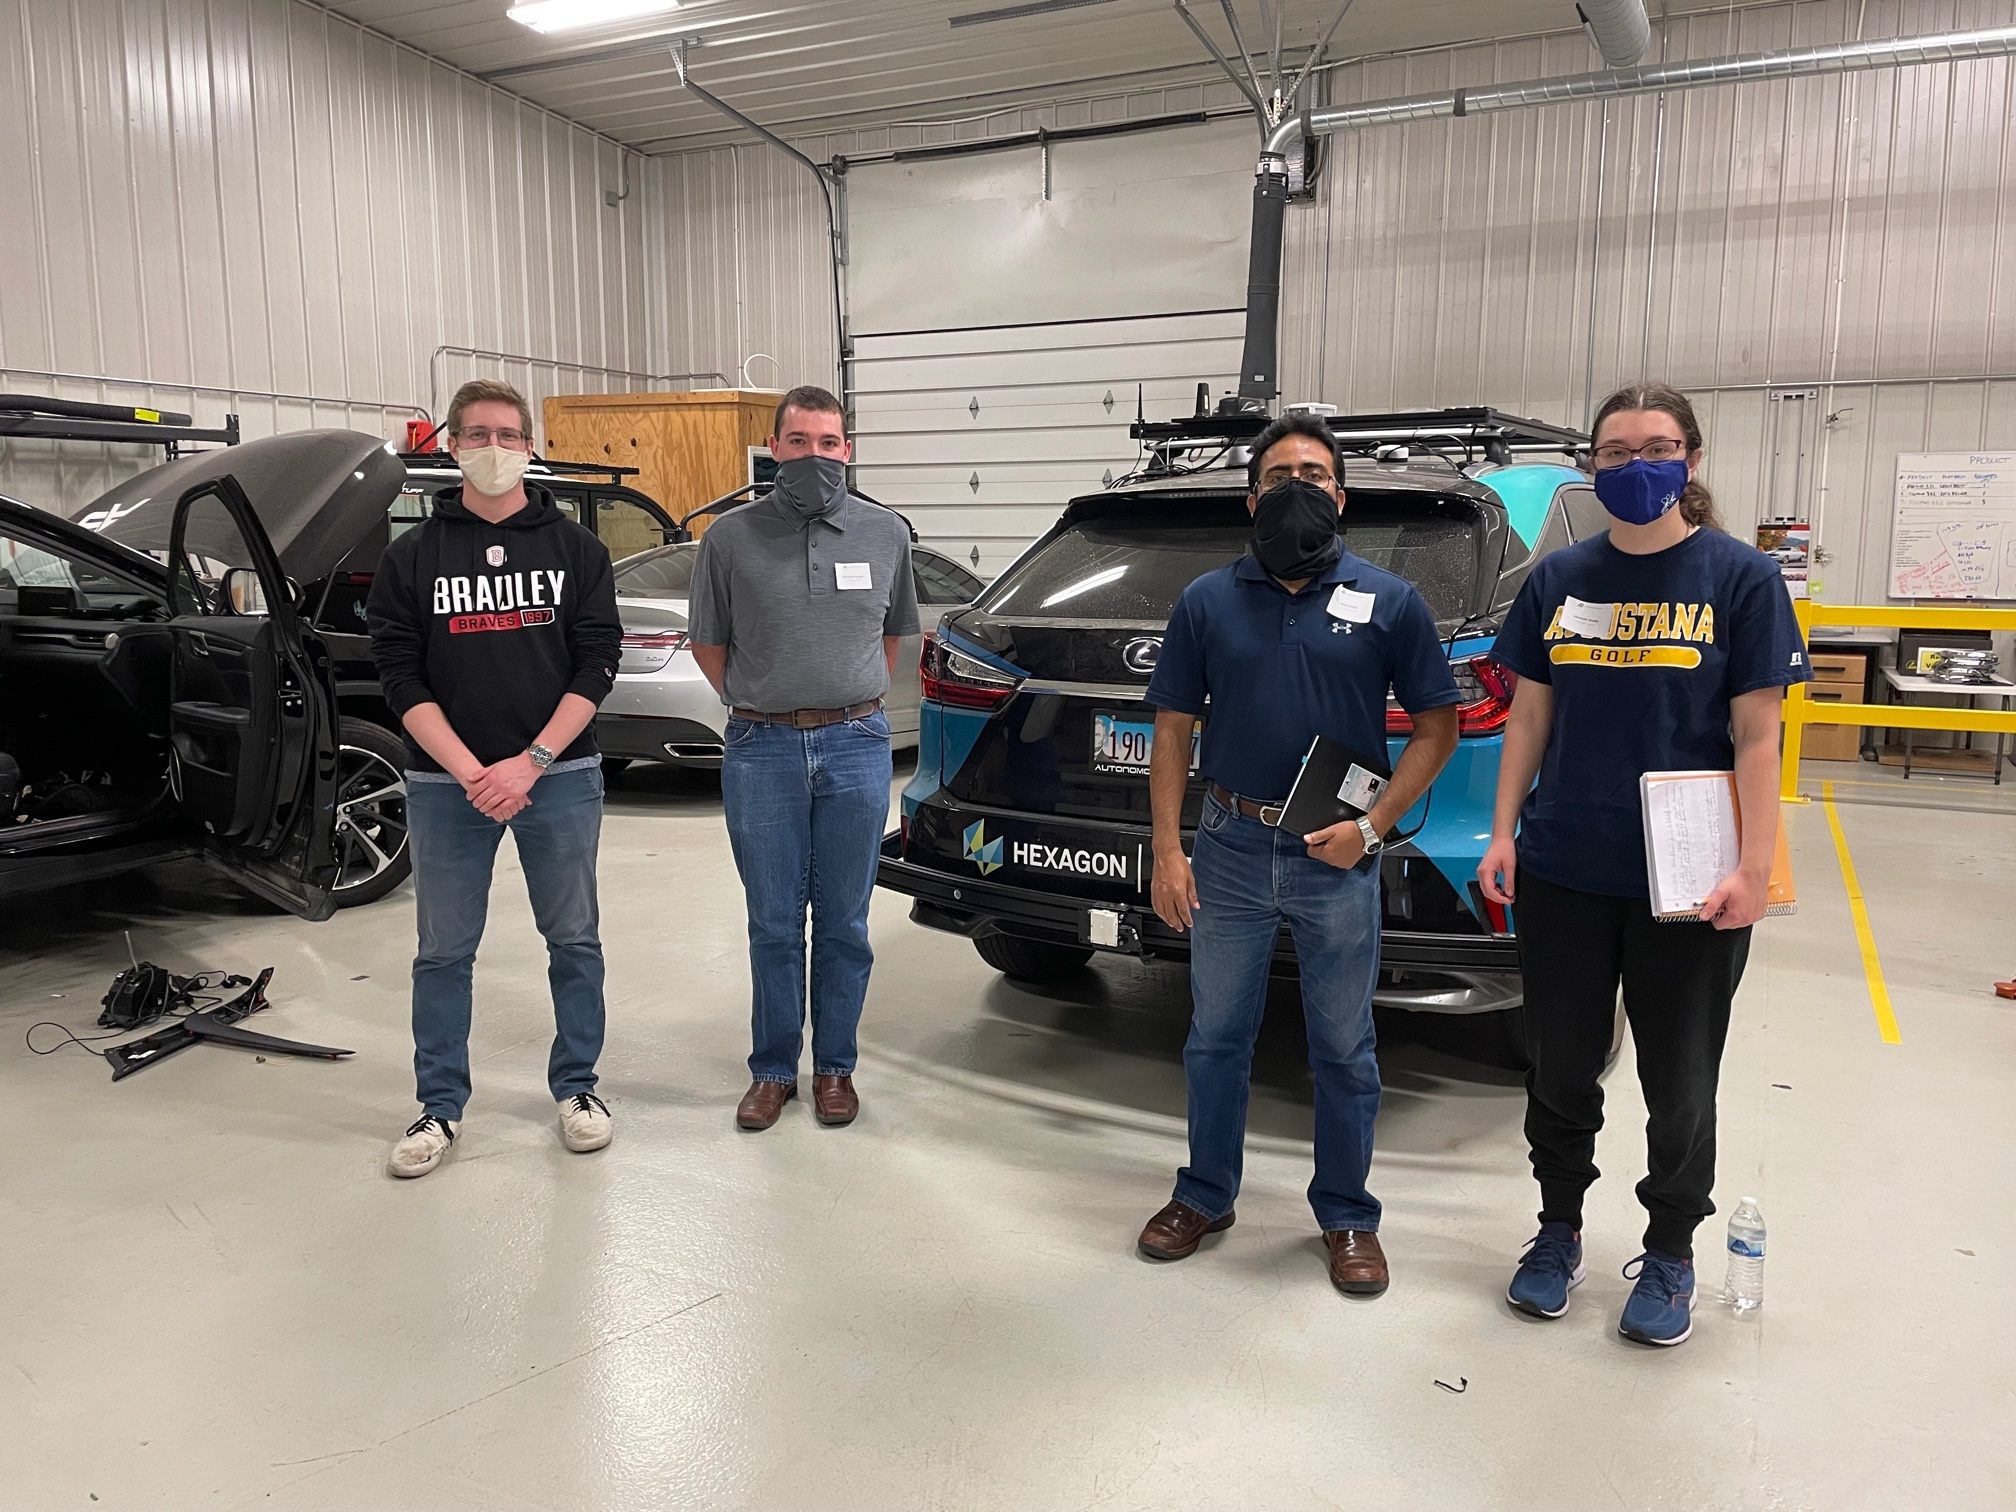
\includegraphics[height=4cm]{figs/img/picturesVisitToAStuff/visitors1-20211007}
	\caption{AutonomouStuff Lexus RX450H vehicle.}
	\label{fig:lexusvehicle}
\end{figure}

\subsection{Steering Subsystem}
\label{sec:steeringSubsystem}

The steering subsystem consists of steering, the power steering motors, $\ldots$ The ultimate goal of this subsystem is to control the steering angle for the vehicle to navigate in the desired heading. Therefore, the control system is designed to produce appropriate voltages to be applied to the power steering motors for the steering orient in the target direction. The block diagram of the control system designed for this subsystem is shown in Fig.~\ref{fig:steeringModelBlockDiagram}


\begin{figure}[h]
  \centering
  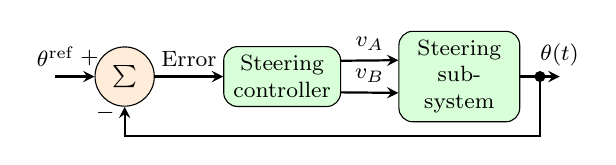
\begin{tikzpicture}
    \tikzstyle{every node} = [font=\footnotesize]
    \tikzstyle{block} = [draw, rectangle, fill=green!15, rounded corners=5pt, minimum width=1 cm, minimum height=0.75 cm]
    \tikzstyle{sum} = [draw, circle,fill=orange!15]
    % place nodes
    \node[sum](sum){$\sum$};
    \node[block,right of=sum,node distance=2 cm, text width=1.25cm,text centered](steeringController){Steering controller};
    \node[block,right of=steeringController,node distance=2.25 cm, text width=1.3cm,text centered](steeringSubsystem){Steering subsystem};

    % Connections
    \draw[stealth-,thick]
    (sum.west)--node[very near start,above]{$+$}++(-0.5,0)node[above]{$\theta^{\text{ref}}$};
    \draw[-stealth,thick]
    (sum.east)--node[midway,above]{Error}(steeringController);
    \draw[-stealth,thick]
    (steeringController.15)--node[midway,above]{$v_A$}(steeringSubsystem.165);
    \draw[-stealth,thick]
    (steeringController.-15)--node[midway,above]{$v_B$}(steeringSubsystem.-165);
    \draw[-stealth,thick]
    (steeringSubsystem.east) --coordinate (tt) ++(0.5,0)node[above]{$\theta(t)$};
    \fill
    ($(steeringSubsystem.east)+(0.25,0)$) circle [radius=2pt];
    \draw[-stealth,thick]
    (tt) -- ++(0,-0.75) -|(sum.south)node[pos=0.9,left]{$-$};
    
  \end{tikzpicture}
  % \captionsetup{justification=centering, margin=3cm}

  % 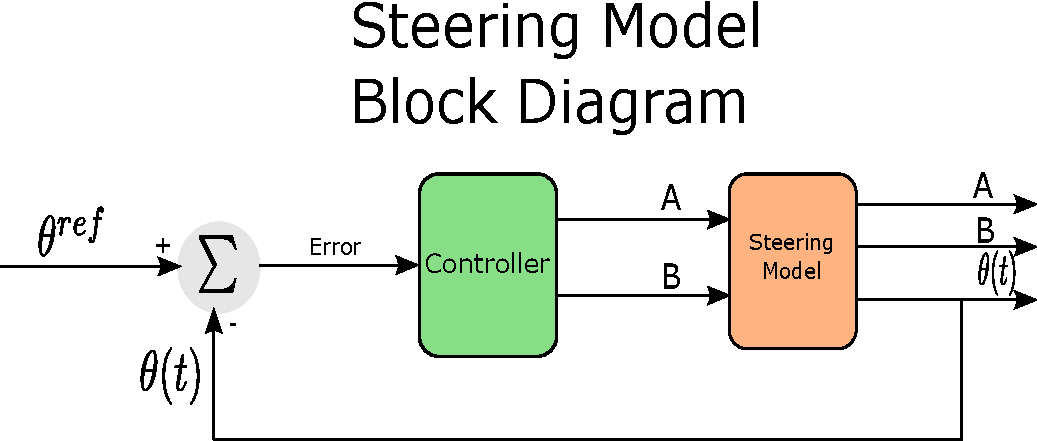
\includegraphics[width=2.5in]{figs/inkscape/steeringModelBlockDiagram}
  \caption{Steering subsystem block diagram.}
  \label{fig:steeringModelBlockDiagram}
\end{figure}


  \subsection{Brake Subsystem}
  The brake subsystem takes the Brake Pedal Pressure Voltages, Brake Pedal Stroke Voltages, and the Brake Pedal On/Off Switch values as inputs. Using these values, it generates a new Brake Pedal Position and a boolean value called Brake Pressed. This boolean value indicates to the user whether or not the brake pedal is being pressed. The brake subsystem is another example of a multiple-input multiple-output system. 
 \begin{figure}[htbp]
    \centering
  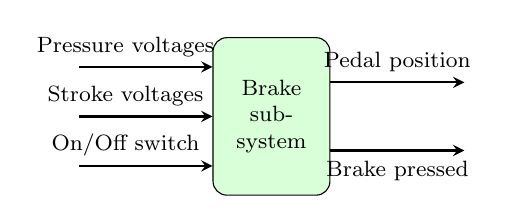
\begin{tikzpicture}
    \tikzstyle{every node} = [font=\footnotesize]
    \tikzstyle{block} = [draw, rectangle, fill=green!15, rounded corners=5pt, minimum width=1 cm, minimum height=2.0 cm]
    % place nodes
    \node[block,text width=1.25cm,text centered](brakeSubsystem){Brake subsystem};

    % Connections
    \draw[stealth-,thick]
    (brakeSubsystem.140)--node[pos=0.65,above]{Pressure voltages}++(-1.7,0);
    \draw[stealth-,thick]
    (brakeSubsystem.180)--node[pos=0.65,above]{Stroke voltages}++(-1.7,0);
    \draw[stealth-,thick]
    (brakeSubsystem.-140)--node[pos=0.65,above]{On/Off switch}++(-1.7,0);
    \draw[-stealth,thick]
    (brakeSubsystem.30)--node[pos=0.5,above]{Pedal position}++(1.7,0);
    \draw[-stealth,thick]
    (brakeSubsystem.-30)--node[pos=0.5,below]{Brake pressed}++(1.7,0);
    
  \end{tikzpicture}
    % \captionsetup{justification=centering, margin=3cm}
    % \includegraphics[width=2.5in]{figs/inkscape/brakeModelArchitecture}
    \caption{Brake subsystem block diagram}
    \label{fig:brakeModelArchitecture}
\end{figure}
 
  \subsection{Acceleration Subsystem}
  The acceleration subsystem is a multiple-input multiple-output system. 
Acceleration pedal voltages are sent to the subsystem. 
A new acceleration pedal position value is generated to better match 
the real-time pedal position. This is then the output 
of the acceleration subsystem. %
%
 \begin{figure}[htbp]
    \centering
  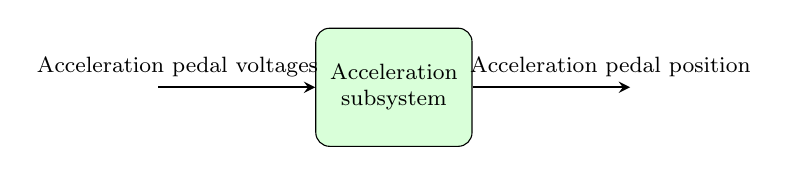
\begin{tikzpicture}
    \tikzstyle{every node} = [font=\footnotesize]
    \tikzstyle{block} = [draw, rectangle, fill=green!15, rounded corners=5pt, minimum width=1.5 cm, minimum height=1.5 cm]
    % place nodes
    \node[block,text width=1.75cm,text centered](accelSubsystem){Acceleration subsystem};
    % Connections
    \draw[stealth-,thick]
    (accelSubsystem.180)--node[very near end,above]{Acceleration pedal voltages}++(-2.0,0);
    \draw[-stealth,thick]
    (accelSubsystem.0)--node[very near end,above]{Acceleration pedal position}++(2.0,0);
  \end{tikzpicture}
    \caption{Acceleration subsystem block diagram}
    \label{fig:accelModelArchitecture}
 \end{figure}
 
  \subsection{Shift Subsystem}
 This subsystem can be classified as a single-input single-output system. The subsystem takes the desired shifter gear value from the user. Within the subsystem, the actual shifter gear changes to better reflect the desired gear. This actual shifter gear value is then the output of the shift subsystem. 
 \begin{figure}[htbp]
    \centering
  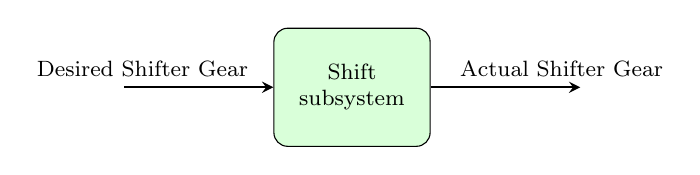
\begin{tikzpicture}
    \tikzstyle{every node} = [font=\footnotesize]
    \tikzstyle{block} = [draw, rectangle, fill=green!15, rounded corners=5pt, minimum width=1.5 cm, minimum height=1.5 cm]
    % place nodes
    \node[block,text width=1.75cm,text centered](shiftSubsystem){Shift subsystem};

    % Connections
    \draw[stealth-,thick]
    (shiftSubsystem.180)--node[very near end,above]{Desired Shifter Gear}++(-1.9,0);
    \draw[-stealth,thick]
    (shiftSubsystem.0)--node[very near end,above]{Actual Shifter Gear}++(1.9,0);
    
  \end{tikzpicture}
    \caption{Shift subsystem block diagram}
    \label{fig:shiftModelArchitecture}
 \end{figure} 
 
  \subsection{Speed Subsystem}
This speed subsystem would fall under the multiple-input single-output system. There are four inputs, the position of the acceleration pedal and the brake pedal, along with the shifter actual gear. Taking these inputs, the speed subsystem finds the vehicle speed. This vehicle speed is then the output of the system.  
 \begin{figure}[htbp]
    \centering
  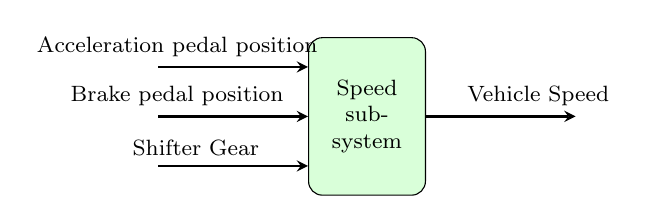
\begin{tikzpicture}
    \tikzstyle{every node} = [font=\footnotesize]
    \tikzstyle{block} = [draw, rectangle, fill=green!15, rounded corners=5pt, minimum width=1 cm, minimum height=2 cm]
    % place nodes
    \node[block,text width=1.25cm,text centered](speedSubsystem){Speed subsystem};

    % Connections
    \draw[stealth-,thick]
    (speedSubsystem.140)--node[very near end,above]{Acceleration pedal position}++(-1.9,0);
    \draw[stealth-,thick]
    (speedSubsystem.180)--node[very near end,above]{Brake pedal position}++(-1.9,0);
    \draw[stealth-,thick]
    (speedSubsystem.-140)--node[near end,above]{Shifter Gear}++(-1.9,0);
    \draw[-stealth,thick]
    (speedSubsystem.0)--node[near end,above]{Vehicle Speed}++(1.9,0);
    
  \end{tikzpicture}
    % \captionsetup{justification=centering, margin=3cm}
    % \includegraphics[width=2.5in]{figs/inkscape/brakeModelArchitecture}
    \caption{Speed subsystem block diagram}
    \label{fig:speedModelArchitecture}
\end{figure}
 
  \subsection{Speed Control Subsystem}
  The speed control subsystem is a straightforward single-input single-output system. The desired vehicle speed is set by the user and sent to the speed control subsystem. Taking this input, the subsystem calculates the new vehicle speed. This value is then sent out to the rest of the vehicle system. 
 \begin{figure}[htbp]
    \centering
  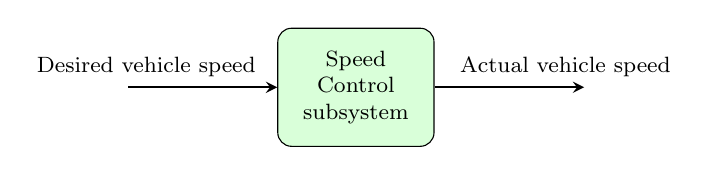
\begin{tikzpicture}
    \tikzstyle{every node} = [font=\footnotesize]
    \tikzstyle{block} = [draw, rectangle, fill=green!15, rounded corners=5pt, minimum width=1.5 cm, minimum height=1.5 cm]
    % place nodes
    \node[block,text width=1.75cm,text centered](speedControlSubsystem){Speed Control subsystem};

    % Connections
    \draw[stealth-,thick]
    (speedControlSubsystem.180)--node[very near end,above]{Desired vehicle speed}++(-1.9,0);
    \draw[-stealth,thick]
    (speedControlSubsystem.0)--node[very near end,above]{Actual vehicle speed}++(1.9,0);
    
  \end{tikzpicture}
    \caption{Speed Control subsystem block diagram}
    \label{fig:speedControlModelArchitecture}
 \end{figure}



 \section{Modeling Dynamic Systems using Neural Networks}

 In this section, we illustrate how a neural network can be used to model a
 dynamic system in general. Neural network is a system approximation technique
 that utilizes the Universal Approximation Theorem, which states that any neural network architecture
 can find a mathematical function $y=f(x)$ that maps inputs $x$ to outputs $y$. The architecture of the 
 neural network and the complexity of the dataset employed affect the accuracy of the function. This theorem
 shows that there will be a determinable function from some neural network architecture and this theorem holds
 for any number of inputs and outputs, like the system show in Fig.~\ref{fig:mimoDynamicBlockDiagram}. 
 The main structure of a neural network consists of neurons, input layer of
 neurons, one or more hidden layers, and the output layer of neurons. The
 neurons of the hidden layers and the output layer have processing capabilities.
 The actual structure of a neural network follows parallel and distributed system
 architecture.

 \begin{figure}[htbp]
    \centering
  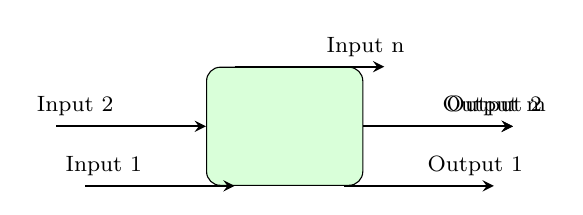
\begin{tikzpicture}
    \tikzstyle{every node} = [font=\footnotesize]
    \tikzstyle{block} = [draw, rectangle, fill=green!15, rounded corners=5pt, minimum width=1.5 cm, minimum height=1.5 cm]
    % place nodes
    \node[block,text width=1.75cm,text centered](plant){};

    % Connections
	\draw[stealth-,thick]
    (plant.-130)--node[very near end,above](in1){Input 1}++(-1.9,0);    
    \draw[stealth-,thick]
    (plant.180)--node[very near end,above](in2){Input 2}++(-1.9,0);
    %\draw[ultra thick,Dotted] (in2) -- (inn);
    \draw[-stealth,thick]
    (plant.130)--node[very near end,above](inn){Input n}++(1.9,0);
    
    \draw[-stealth,thick]
    (plant.-45)--node[very near end,above](out1){Output 1}++(1.9,0);
    \draw[-stealth,thick]
    (plant.0)--node[very near end,above](out2){Output 2}++(1.9,0);
    %\draw[ultra thick,Dotted] (out2) -- (outm);
    \draw[-stealth,thick]
    (plant.0)--node[very near end,above](outm){Output m}++(1.9,0);
    
    
  \end{tikzpicture}
    \caption{Multiple Input Multiple Output Dynamic System Block Diagram}
    \label{fig:mimoDynamicBlockDiagram}
 \end{figure}
 
 Figure~\ref{fig:nnActor} shows a generic actor neural network structure. ...
 \begin{figure}
  \centering
      \tikzset{%
        input neuron/.style={
          circle,
          fill=green!50,
          minimum size=0.7cm
        },
        neuron missing/.style={
          draw=none, 
          scale=1,
          fill=white,
          text height=0.01cm,
          execute at begin node=\color{black}$\vdots$
        },
      }

      \tikzset{%
        hidden neuron/.style={
          circle,
          fill=blue!50,
          minimum size=0.7cm
        },
        neuron missing/.style={
          draw=none, 
          scale=1,
          fill=white,
          text height=0.01cm,
          execute at begin node=\color{black}$\vdots$
        },
      }

      \tikzset{%
        output neuron/.style={
          circle,
          fill=red!50,
          minimum size=0.7cm
        },
        neuron missing/.style={
          draw=none, 
          scale=1,
          fill=white,
          text height=0.01cm,
          execute at begin node=\color{black}$\vdots$
        },
      }      

      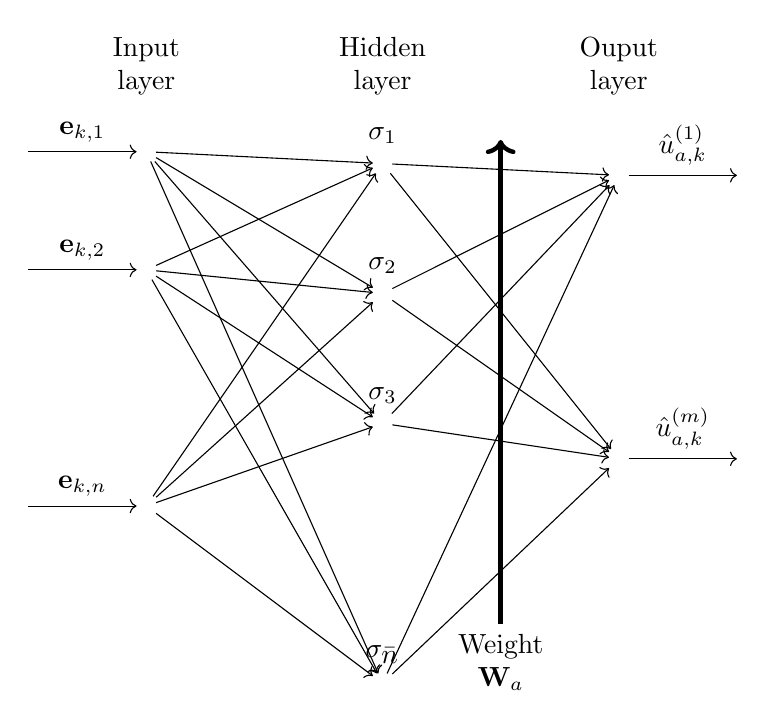
\begin{tikzpicture}[x=1.5cm, y=1.5cm]

        \foreach \m/\l [count=\y] in {1,2,missing,3}
        \node [input neuron/.try, neuron \m/.try] (input-\m) at (0,2.5-\y) {};

        \foreach \m [count=\y] in {1,2,3,missing,4}
        \node [hidden neuron/.try, neuron \m/.try ] (hidden-\m) at (2,2.5-\y*1.1) {};

        \foreach \m [count=\y] in {1,missing,2}
        \node [output neuron/.try, neuron \m/.try] (output-\m) at (4,2.5-\y*1.2) {};

        \foreach \l [count=\i] in {1,2,n}
        \draw [<-] (input-\i) -- ++(-1,0)
        node [above, midway] {$\mathbf{e}_{k,\l}$};

        \foreach \l [count=\i] in {1,2,3,\mbox{$\bar{n}$}}
        \node [above] at (hidden-\i.north) {$\sigma_{\l}$};

        \foreach \l [count=\i] in {1,m}
        \draw [->] (output-\i) -- ++(1,0)
        node [above, midway] {$\hat{u}_{a,k}^{(\l)}$};

        \foreach \i in {1,...,3}
        \foreach \j in {1,...,4}
        \draw [->] (input-\i) -- (hidden-\j);

        \foreach \i in {1,...,4}
        \foreach \j in {1,2}
        \draw [->] (hidden-\i) -- (output-\j);


        
        \foreach \l [count=\x from 0] in {Input, Hidden, Ouput}
        \node [align=center, above] at (\x*2,1.9) {\l \\ layer};

        \node [align=center, below] at (3,-2.5) {Weight \\ $\mathbf{W}_a$};
        \draw[->,ultra thick](3,-2.5) -- (3,1.6);
        
      \end{tikzpicture}
  \caption{Actor neural network structure for approximating control input.}
  \label{fig:nnActor}
\end{figure}

 \todo[inline]{Weights of a neural network}

 \todo[inline]{Training of a neural network}
 \todo[inline]{Testing a neural network}
 
 

\section{Modeling Vehicle Subsystems}

To start the project, we researched methods of plant modeling for autonomous vehicles and more generically, nonlinear systems. From our research, we found a few methods of modeling that we employed to discover the most accurate representation of each vehicle subsystem. The first method that we tried was developing different system types using Mathworks' MATLAB System Identification Toolbox. Using data we collected from the Lexus vehcile platform at AutonomouStuff,this toolbox allowed us to add input and output data for each vehicle subsystem. With this data, we used one subset to train the system and another subset for validation. Using this toolbox, we tried developing state-space models, NARX models, and transfer function models. We also used Mathworks' MATLAB Neural Network Time Series toolbox to develop a model of each vehicle subsystem using neural network modeling making use of the Bayesian Regularization training method. The following requirements were used to evaluate the effectiveness of our models to determine which plant model should be presented to AutonomouStuff.


\subsection{System Requirements}

In order to accurately model each vehicle subsystem so that safe, reliable controllers can be developed for autonomous control, the following criteria will be met:
\begin{itemize}
\item Each vehicle subsystem will be able to track nonlinearities depicted in Fig.~\ref{fig:nonlinGraph} associated with small changes in the output of each subsystem
\item Each vehicle subsystem plant model will track any desired inputs within the specified error bounds
	\begin{itemize}
		\item Steering Angle within 5 degrees
		\item Pedal Positions within 5\%
	\end{itemize}
\item Each vehicle subsystem will be modeled independently from other vehicle subsystems
\end{itemize}

The vehicle plant model will fulfill the requirements listed below:
\begin{itemize}
    \item The resulting plant model will consist of accurate subsystem models, as defined above
    \item The subsystems can be used to create a HIL testbench
    \item The subsystems can handle very small changes in their output accurately
\end{itemize}

All of the subsystems have nonlinear behaviors when there are small changes in the output of the subsystem. The steering subsystem, for example, should behave in a smooth, continuous manner. However, AutonomouStuff observed that when trying to implement features such as lane tracking for the Lexus vehicle platform, that when small changes in the steering angle (less than five degrees) occurred, the torque voltages would momentarily stall and then suddenly change causing a more drastic change. This behavior, depicted in Fig.~\ref{fig:nonlinGraph}, made it very challenging to complete features like lane tracking. These models will aid in the development of controllers that will remove the nonlinearities allowing features like lane tracking to be implemented in a safer, smoother manner. 

\begin{figure}[htbp]
    \centering
    \captionsetup{justification=centering}
    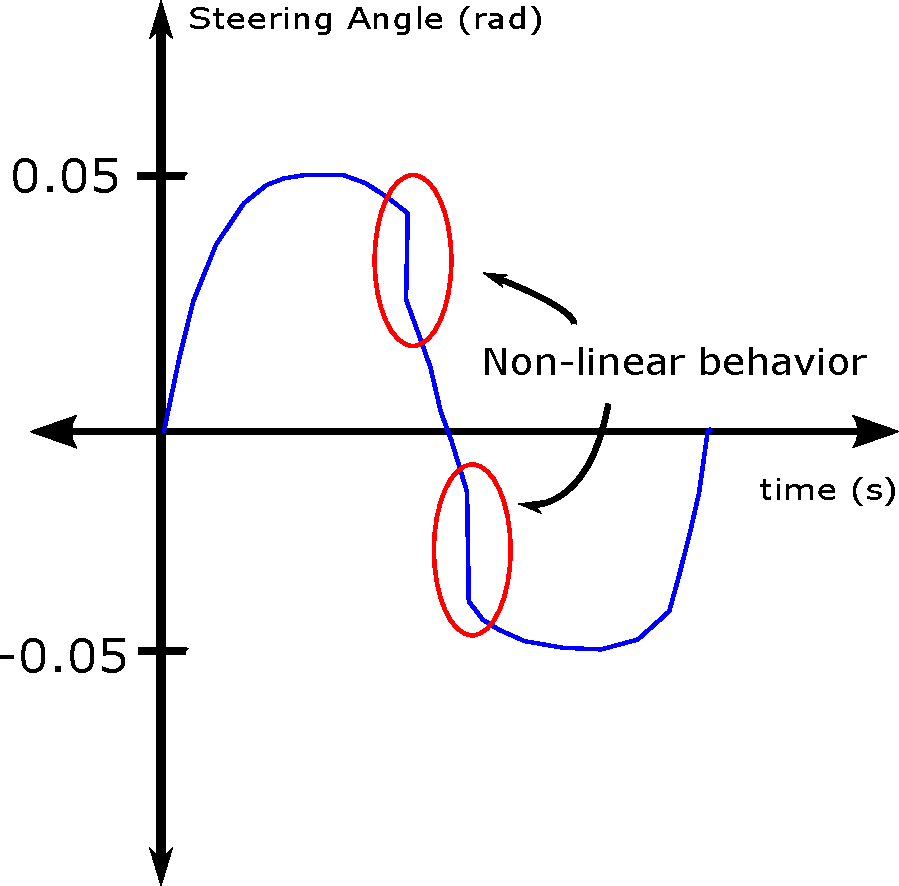
\includegraphics[width=2.5in]{figs/inkscape/nonlinearBehavior}
    \caption{Steering Non-linear Behavior}
    \label{fig:nonlinGraph}
\end{figure}

\subsection{Steering System Modeling}
To develop a model of the steering system, we employed multiple methods. The first method that we tried was generating a NARX model and a transfer function model, making use of the System Identification Toolbox in MATLAB. The NARX model we developed was not accurate and did not track the output of the steering system data. The transfer function model we developed was more reliable tracking the output of the steering system data, but was unable to meet the error requirements, as there were sudden changes that forced high error peaks. Then we employed a neural network model, making use of the Neural Network Time Series Toolbox in MATLAB. With the neural network model, the model was able to reliably and accurately track the output of the steering system data and stayed within the error requirements. 

\subsection{Acceleration System Modeling}
To develop a model of the acceleration system, we employed multiple methods. The first method that we tried was generating a NARX model and a transfer function model, making use of the System Identification Toolbox in MATLAB. The NARX model we developed was not accurate and did not track the output of the acceleration system data. The transfer function model we developed was more reliable tracking the output of the acceleration system data, but was unable to meet the error requirements, as there were sudden changes that forced high error peaks. Then we employed a neural network model, making use of the Neural Network Time Series Toolbox in MATLAB. With the neural network model, the model was able to reliably and accurately track the output of the acceleration system data and stayed within the error requirements. 

\subsection{Brake System Modeling}
To create a brake system model, we first tried generating transfer function models using MATLAB’s System Identification Toolbox. After generating multiple transfer function models and trying many different data log combinations, we still couldn’t find a model that was completely accurate across all combinations and that was below the error bound of 5\% for all combinations. Once this became clear Neural Network models were created using the Neural Network Time Series Toolbox provided by MATLAB to see if they could create accurate brake models. Using this we were able to create a model that accurately tracked the data we collected from the brake system and that stayed within the 5\% error bound.  

\todo[inline]{Add subsections for each subsystem on how NNs are used to model each subsystem}

\todo[inline]{For each subsystem you will need to draw different NN structure }



\section{Validation and Testing} \label{sec:simresults}


%To start this project, we first read documentation outlining the uses of
%MATLAB's System Identification Toolbox. From there we worked on MATLAB tutorials
%on how to model systems from data using System Identification and then find the
%most accurate model. We specifically tried to find examples with Multiple-Input
%Multiple-Output (MIMO) and Multiple-Input Single-Output (MISO) systems, since
%most of the vehicle subsystems we will model fall into one of these categories.
%A literature review was also conducted to see how systems with small
%non-linearities like our steering subsystem were modeled using System
%Identification.

\subsection{Experimental Setup}
\label{sec:experimentalSetup}

We traveled to AutonomouStuff in order to collect
data from the steering, acceleration, and braking subsystems in an autonomous
vehicle. The data we collected will be used to generate and then verify our
models. We collected data on the Lexus RX450H vehicle platform shown in
Fig.~\ref{fig:lexusvehicle}. %


\noindent The following is the hardware components required to collect the data:  
	\begin{itemize}
    		\item Laptop
    		\item PACMod ECU
    		\item CANCase 
    		\item CAN bus 
 	\end{itemize}
 	
 	
\noindent The laptop is used to pass commands or log data, such as steering angle or acceleration or brake pedal position. This data is sent or received using the CANCase and CAN bus. These are connected to the AutonomouStuff designed PACMod ECU, which sends torque voltages to the desired vehicle subsystem allowing the laptop to either control the desired vehicle system or log data. The Vector CANAlyzer software is installed on the laptop and is used to parse the collected data that is sent from the CANCase. This is how we were able to collect logs of data that we would use to develop models of the autonomous vehicle subsystems.
\\

Each subsystem that we are modeling is set up in a similar manner. In manual mode, the torque voltages that control each subsystem are sent by the vehicle's electronic control unit (ECU). In order to control the vehicle autonomously, the vehicle subsystem switches to by-wire mode. In by-wire mode, the torque voltages from the vehicle's ECU are discarded by open-circuiting the motors that control each subsystem. Instead, the PACMod ECU built by AutonomouStuff sends the torque voltages to the motor using relays. In Fig.~\ref{fig:vehicleSetup}, the experimental setup for data collection is shown. The laptop is used to collect the data from the desired vehicle subsystem by the use of Vector's CANAlyzer software. The CAN Case collects data from the PAC Mod and ECU and sends the data using a CAN bus to the laptop which is then parsed and displayed through the use of CANAlyzer. The ECU and PAC Mod are not shown in Fig.~\ref{fig:vehicleSetup} as they are fixed behind panels of the vehicle. 
\\

\begin{figure}[htbp]
	\centering
    	% \captionsetup{justification=centering, margin=3cm}
    	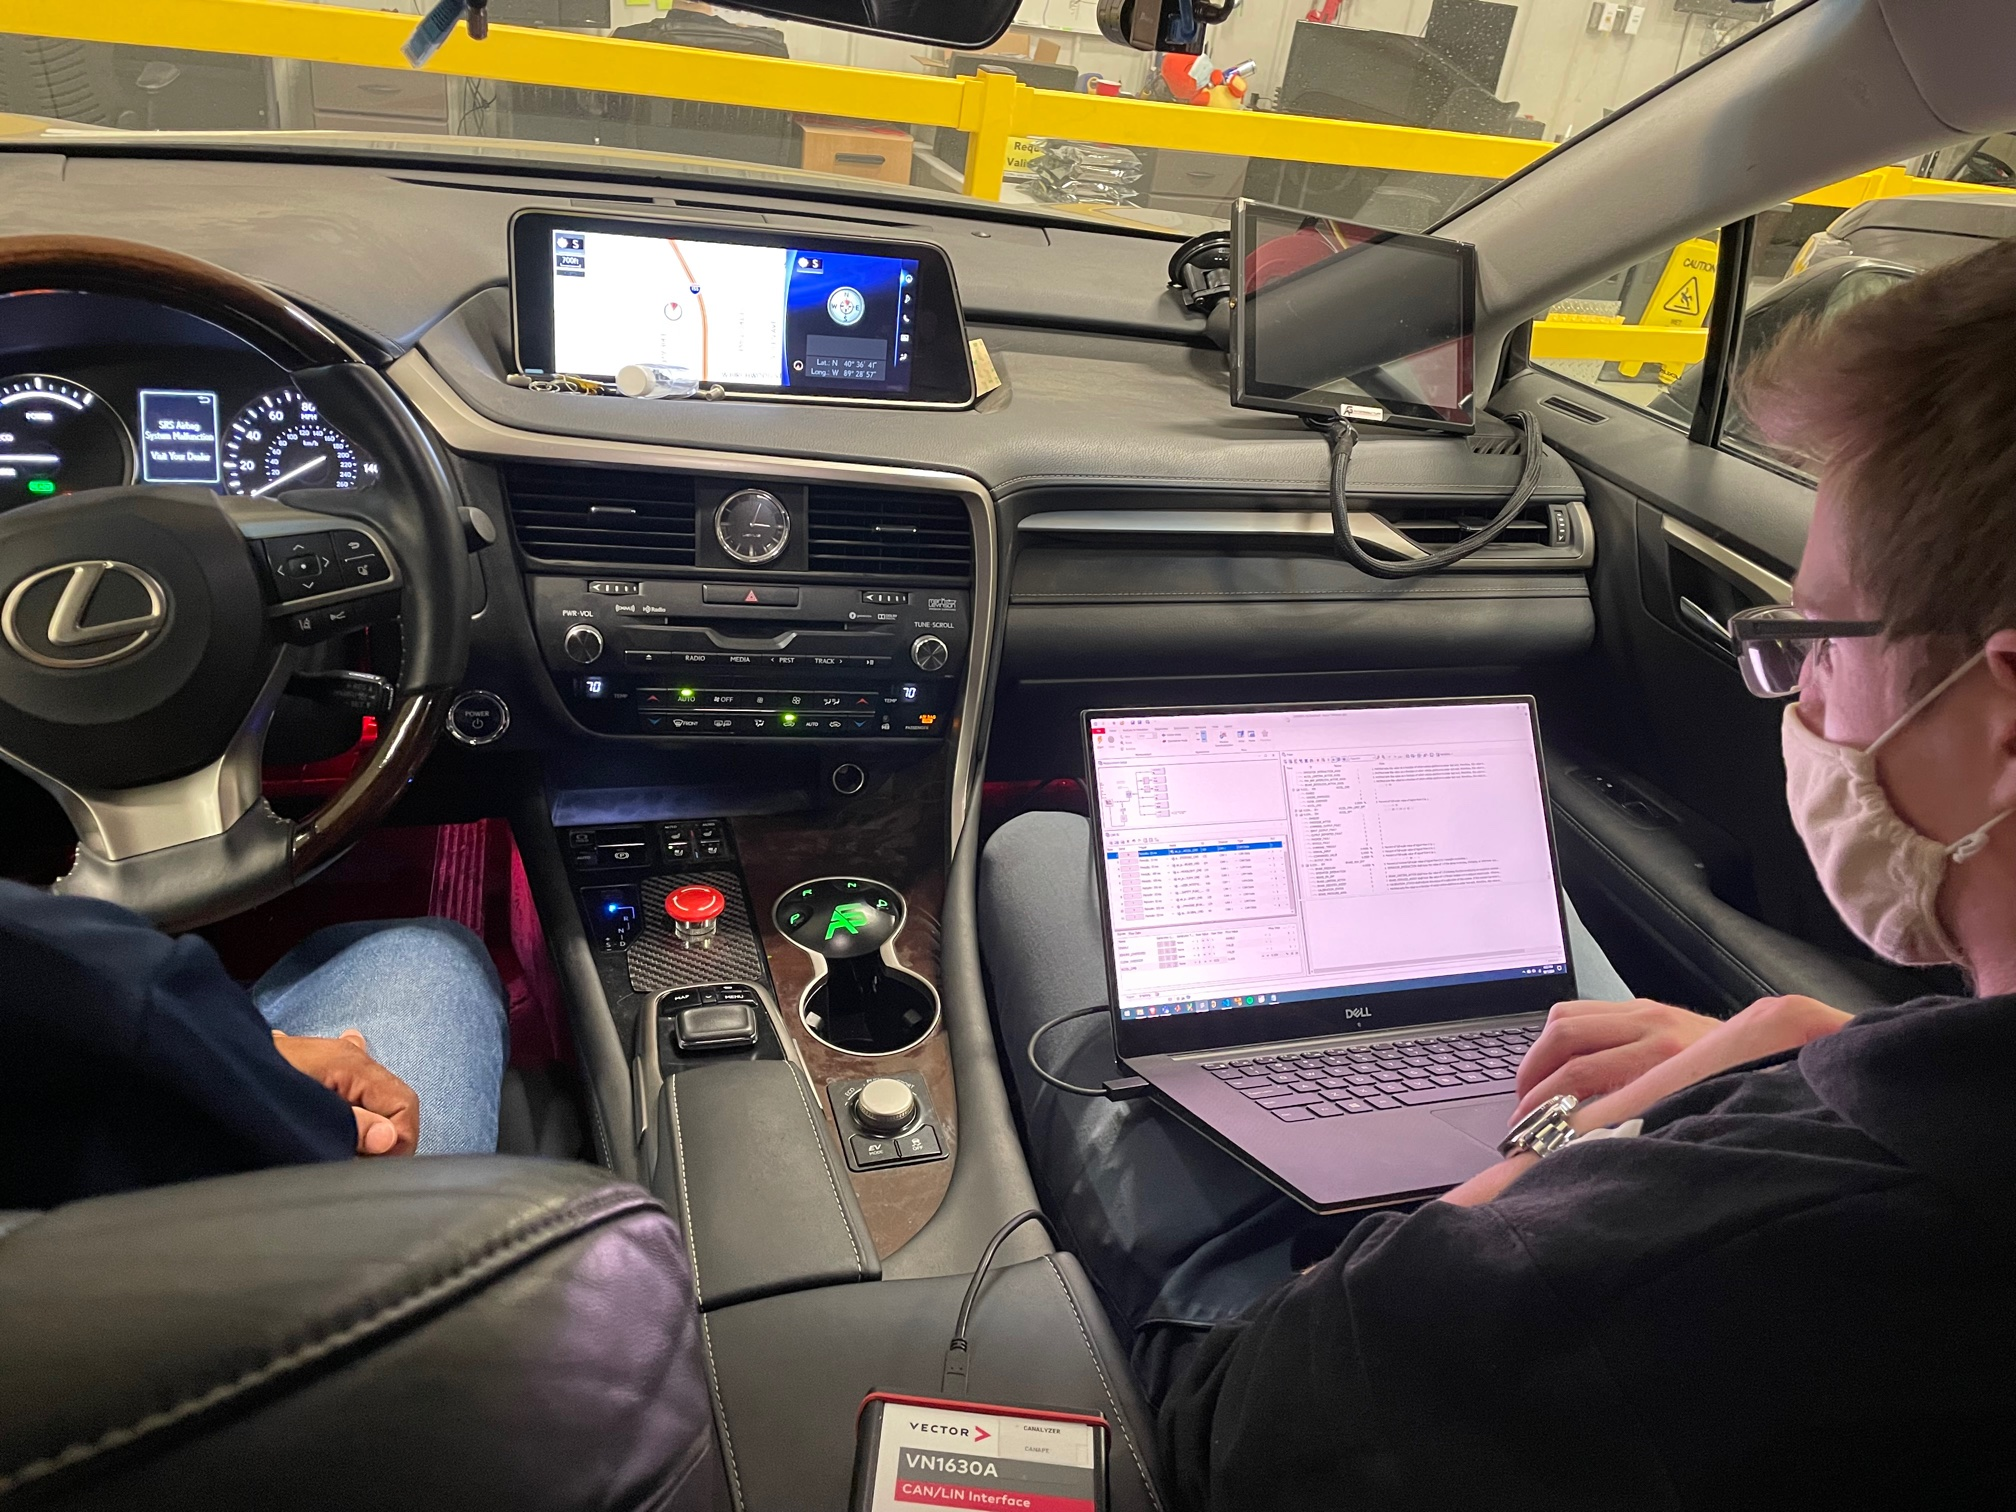
\includegraphics[width=.48\textwidth]{figs/img/picturesVisitToAStuff/dataColletionSetup1-20211007}
    	\caption{Autonomous Vehicle Data Collection Setup}
    	\label{fig:vehicleSetup}
\end{figure}

Using the data we collected for the steering, acceleration, and braking subsystems, we initially separated the data so we could analyze the by-wire and manual modes individually. This effort was made to identify if the models we developed could be used interchangeably regardless of what mode the autonomous vehicle subsystems were operating in. After analyzing the models we developed, we determined that they are not interchangeable as there were differences in the models. When the vehicle subsystem is in by-wire mode, the controller AutonomouStuff developed is generating the torque voltages that are applied to each subsystem motor. As a result, we decided the most accurate model of each subsystem would be developed using the data when the subsystems are in manual mode. For reference, the differences in the models created for by-wire and manual mode are depicted in \ref{sec:simresults} for the steering and acceleration subsystems. For all other models we develop, we will only use manual mode data and will not create models for by-wire mode.


\subsection{Transfer Function Modeling}
\label{sec:TransferFunctionModeling}

\todo[inline]{Discuss results using the setup you explained in the previous section. See some IEEE papers}

\subsubsection{Steering Subsystem}
In Fig.~\ref{byWireSteerModel}, the output steering angle is plotted versus time
when the vehicle is in by-wire mode. The figure shows the output steering angle
from some data collected to depict the steering system behavior plotted with the
behavior of the estimated model. The best fit percentage for this model is
85.54\%. Likewise, Fig.~\ref{manualSteerModel} depicts the output steering angle
plotted versus time when the vehicle is in manual mode. The best fit percentage
for this model is 90.27\%.


  % %
  % \begin{figure}
  %   \centering
  %   \begin{subfigure}[b]{0.48\linewidth}
  %     \centering
  %     \includegraphics[width=\textwidth]{figs/fusion360/PowertrainModelCorrectDimsTopViewV3}
  %     \caption{}
  %     \label{fig:PowertrainModelCorrectDimsTopViewV3}
  %   \end{subfigure}
  %   \begin{subfigure}[b]{0.48\linewidth}
  %     \centering
  %     \includegraphics[width=\textwidth]{figs/fusion360/PowertrainModelCorrectDimsFrontViewV4}
  %     \caption{}
  %     \label{fig:PowertrainModelCorrectDimsFrontViewV4}
  %   \end{subfigure}
  %   \begin{subfigure}[b]{0.48\linewidth}
  %     \centering
  %     \includegraphics[width=\textwidth]{figs/fusion360/PowertrainModelCorrectDimsSideViewV4}
  %     \caption{}
  %     \label{fig:PowertrainModelCorrectDimsSideViewV4}
  %   \end{subfigure}
  %   \caption{\subref{fig:PowertrainModelCorrectDimsTopViewV3} Top view,
  %     \subref{fig:PowertrainModelCorrectDimsFrontViewV4} front view, and
  %     \subref{fig:PowertrainModelCorrectDimsSideViewV4} side view of the
  %     proposed disinfecting robot.}
  %   \label{fig:2dViewsDisinfectingRobot}
  % \end{figure}

\begin{figure}[h]
	\centering
	\subcaptionbox{Output of Estimated By-Wire System Model \label{byWireSteerModel}}
		{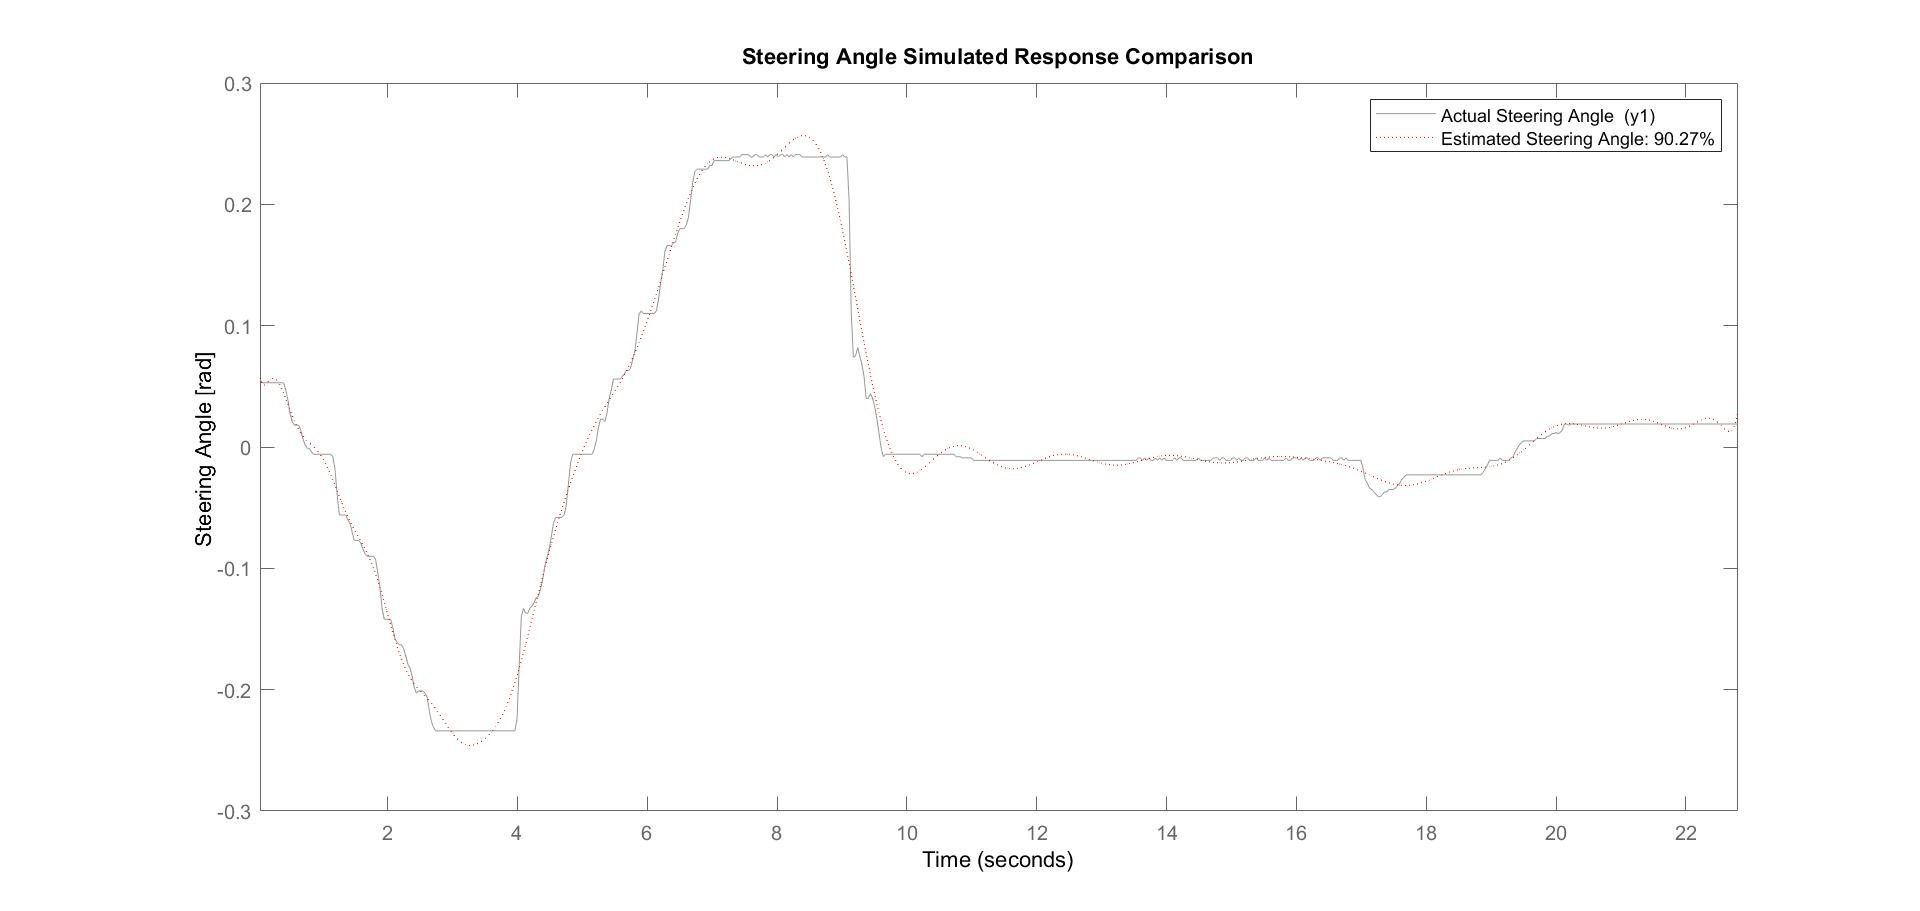
\includegraphics[width=0.48\linewidth]{figs/img/byWireSteeringTransferFunctionModel}}
	\subcaptionbox{Output of Estimated Manual System Model \label{manualSteerModel}}
		{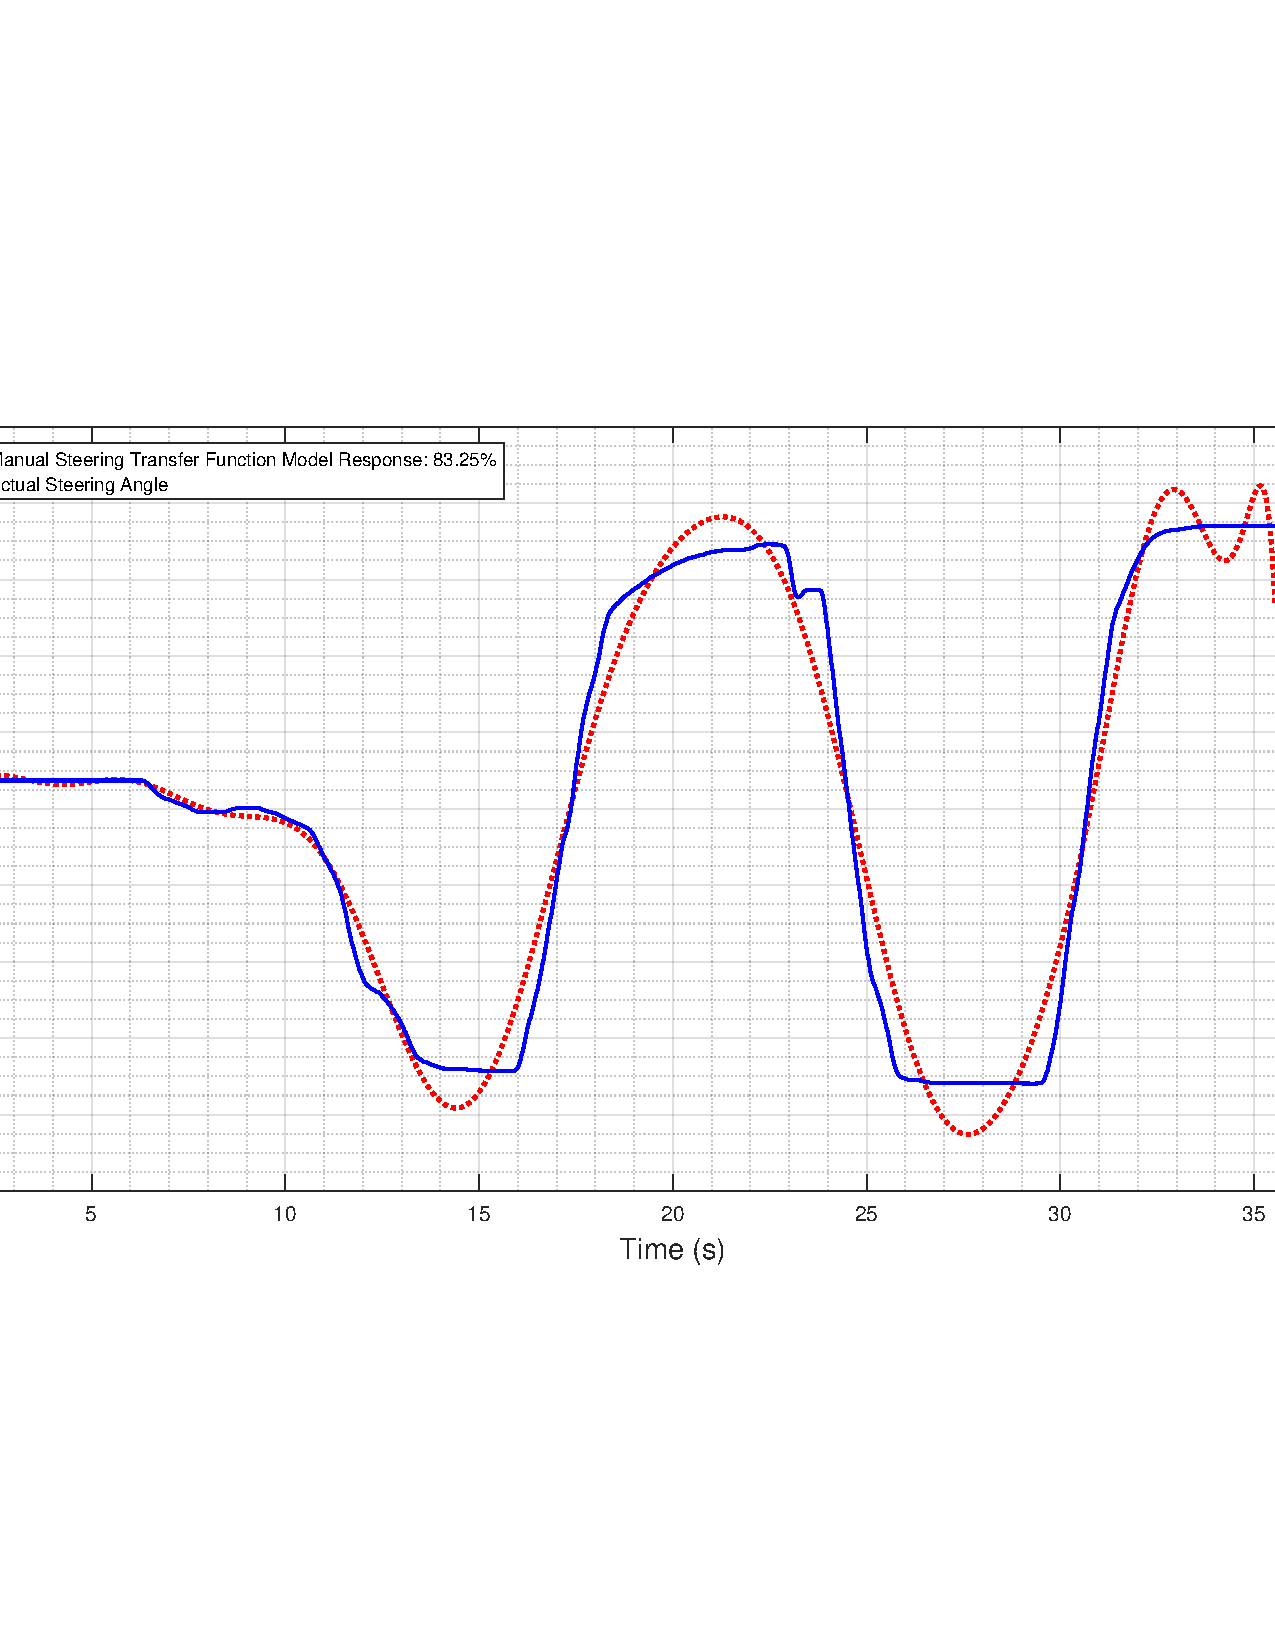
\includegraphics[width=0.48\linewidth]{figs/img/manualSteeringTransferFunctionModel}}
	\caption{Steering System Estimated Steering Angle Comparison}
\end{figure}

\vspace{12pt}
\noindent The model of the by-wire steering system is a twentieth order transfer function. The twentieth order transfer function is the best proposed estimation considering the system costs associated with a higher order transfer function while also obtaining an acceptable best fit percentage. Table~\ref{tab:byWireSteerCoeffA} shows the coefficients of the twentieth order transfer function for the output steering angle with respect to the input torque voltage A signal.%
%
\begin{table}[hbtp]
	\label{tab:byWireSteerCoeffA}
	\caption{By-Wire Mode Steering Transfer Function Torque Voltage A Coefficient Table}
  \centering
  \resizebox{\linewidth}{!}{% Resize table to fit within \linewidth horizontally
    \begin{tabular}{*{21}{c}}
      \toprule
      $a_0$& $a_1$&$a_2$&$a_3$&$a_4$&$a_5$&$a_6$&$a_7$&$a_8$&$a_9$&$a_{10}$&$a_{11}$&$a_{12}$&$a_{13}$&$a_{14}$&$a_{15}$&$a_{16}$&$a_{17}$&$a_{18}$ &$a_{19}$&$a_{20}$\\
      \midrule
      1.949E-16 & 1.455E-14 & 8.797E-13 & 2.304E-11 & 9.041E-10 & 9.01E-9 & 2.714E-7 & 9.241E-7 & 1.946E-5 & 3.889E-5 & 0.0005721 & 0.0008035 & 0.008695 & 0.008922 & 0.07499 & 0.05422 & 0.3631 & 0.1693 & 0.9394 & 0.2118 & 1\\
      \bottomrule
    \end{tabular}}
    
	\begin{center}
		\resizebox{0.4\linewidth}{!}{% Resize table to fit within \linewidth horizontally
    		\begin{tabular}{*{21}{c}}
      	\toprule
      	$b_0$& $b_1$&$b_2$&$b_3$&$b_4$&$b_5$\\
      	\midrule
      	3.44E-16 & -2.203E-15 & 1.24E-13 & 5.975E-13 & 3.001E-12 & 5.23E-12\\
      	\bottomrule
    		\end{tabular}}
	\end{center}	
\end{table}
%
 
\noindent Table~\ref{tab:byWireSteerCoeffB} shows the coefficients of the twentieth order transfer function for the output steering angle with respect to the input torque voltage B signal.%
%
\begin{table}[hbtp]
	\label{tab:byWireSteerCoeffB}
	\caption{By-Wire Mode Steering Transfer Function Torque Voltage B Coefficient Table}
  \centering
  \resizebox{\linewidth}{!}{% Resize table to fit within \linewidth horizontally
    \begin{tabular}{*{21}{c}}
      \toprule
      $a_0$& $a_1$&$a_2$&$a_3$&$a_4$&$a_5$&$a_6$&$a_7$&$a_8$&$a_9$&$a_{10}$&$a_{11}$&$a_{12}$&$a_{13}$&$a_{14}$&$a_{15}$&$a_{16}$&$a_{17}$&$a_{18}$ &$a_{19}$&$a_{20}$\\
      \midrule
      2.92E-15 & 2.758E-13 & 1.761E-11 & 4.228E-10 & 1.422E-8 & 1.561E-7 & 1.501E-6 & 8.426E-6 & 5.981E-5 & 0.0002016 & 0.001226 & 0.002649 & 0.01456 & 0.02044 & 0.104 & 0.09228 & 0.4417 & 0.2257 & 1.025 & 0.2305 & 1\\
      \bottomrule
    \end{tabular}}
	\begin{center}
		\resizebox{0.4\linewidth}{!}{% Resize table to fit within \linewidth horizontally
    		\begin{tabular}{*{21}{c}}
     	 \toprule
     	 $b_0$& $b_1$&$b_2$&$b_3$&$b_4$&$b_5$\\
     	 \midrule
      	-6.645E-15 & 2.161E-14 & -2.605E-14 & -4.744E-13 & -1.813E-13 & -4.858E-12\\
      	\bottomrule
    \end{tabular}}
	\end{center}
\end{table}
%

\vspace{12pt}
\noindent The manual steering system is modeled by a twentieth order transfer
function. After considering the system costs that come with a higher order
transfer function and the need to achieve a sufficient best fit percentage, it
is clear that a twentieth order transfer function is the best estimation of the
system. Table~\ref{tab:manualSteerCoeffA} shows the coefficients of the twentieth
order transfer function for the output steering angle with respect to the input
torque voltage A signal. %
%
  \begin{table}[hbtp]
    \caption{Manual mode steering transfer function torque voltage A coefficient table. }
    \label{tab:manualSteerCoeffA}
    \centering
	  \resizebox{\linewidth}{!}{% Resize table to fit within \linewidth horizontally
      \begin{tabular}{*{21}{c}}
        \toprule
        $a_0$& $a_1$&$a_2$&$a_3$&$a_4$&$a_5$&$a_6$&$a_7$&$a_8$&$a_9$&$a_{10}$&$a_{11}$&$a_{12}$&$a_{13}$&$a_{14}$&$a_{15}$&$a_{16}$&$a_{17}$&$a_{18}$ &$a_{19}$&$a_{20}$\\
        \midrule
        1.224E5 & 4.227E5 & 2.202E6 & 3.54E6 & 7.98E6 & 7.62E5 & 1.071E7 & 6.745E6 & 6.85E6 & 3.006E6 & 2.365E6 & 7.37E5 & 4.669E5 & 1.021E5 & 5.319E4 & 7752 & 3353 & 287.5 & 102.4 & 3.653 & 1\\
        \bottomrule
      \end{tabular}}
    \begin{center}
    	\resizebox{0.4\linewidth}{!}{% Resize table to fit within \linewidth horizontally
        \begin{tabular}{*{21}{c}}
          \toprule
          $b_0$& $b_1$&$b_2$&$b_3$&$b_4$&$b_5$\\
          \midrule
          6.516E4 & -2.944E5 & 2.328E5 & -2.487E5 & 8.25E4 & -3.038E4\\
          \bottomrule
        \end{tabular}}
    \end{center}
  \end{table}
%


\noindent Table~\ref{tab:manualSteerCoeffB} shows the coefficients of
the twentieth order transfer function for the output steering angle with respect
to the input torque voltage B signal. %
%
\begin{table}[hbtp]
	\caption{Manual Mode Steering Transfer Function Torque Voltage B Coefficient Table}
	\label{tab:manualSteerCoeffB}
  \centering
  \resizebox{\linewidth}{!}{% Resize table to fit within \linewidth horizontally
    \begin{tabular}{*{21}{c}}
      \toprule
      $a_0$& $a_1$&$a_2$&$a_3$&$a_4$&$a_5$&$a_6$&$a_7$&$a_8$&$a_9$&$a_{10}$&$a_{11}$&$a_{12}$&$a_{13}$&$a_{14}$&$a_{15}$&$a_{16}$&$a_{17}$&$a_{18}$ &$a_{19}$&$a_{20}$\\
      \midrule
      4.687E4 & 7.037E5 & 2.624E6 & 6.133E6 & 1.197E7 & 1.487E7 & 1.887E7 & 1.446E7 & 1.314E7 & 7.01E6 & 4.79E6 & 1.886E6 & 9.836E5 & 2.937E5 & 1.149E5 & 2.617E4 & 7205 & 1232 & 200 & 23.54 & 1\\
      \bottomrule
    \end{tabular}}
	\begin{center}
    \resizebox{0.4\linewidth}{!}{% Resize table to fit within \linewidth horizontally
      \begin{tabular}{*{21}{c}}
        \toprule
        $b_0$& $b_1$&$b_2$&$b_3$&$b_4$&$b_5$\\
        \midrule
        1.209E4 & 1.855E5 & -2.801E5 & 4.72E5 & -3.976E4 & 7.693E4\\
        \bottomrule
      \end{tabular}}
	\end{center}	
\end{table}
%

\subsubsection{Acceleration System}
In \autoref{byWireAccelModel}, the output acceleration pedal position is plotted versus time when the vehicle is in by-wire mode. The figure shows the output acceleration pedal position from some data collected to depict the acceleration system behavior plotted with the behavior of the estimated model. The best fit percentage for this model is 97.69\%. Likewise, \autoref{manualAccelModel} depicts the output acceleration pedal position plotted versus time when the vehicle is in manual mode. The best fit percentage for this model is 98.3\%. 

\begin{figure}[h]
	\centering
	\subcaptionbox{Output of Estimated By-Wire System Model \label{byWireAccelModel}}
		{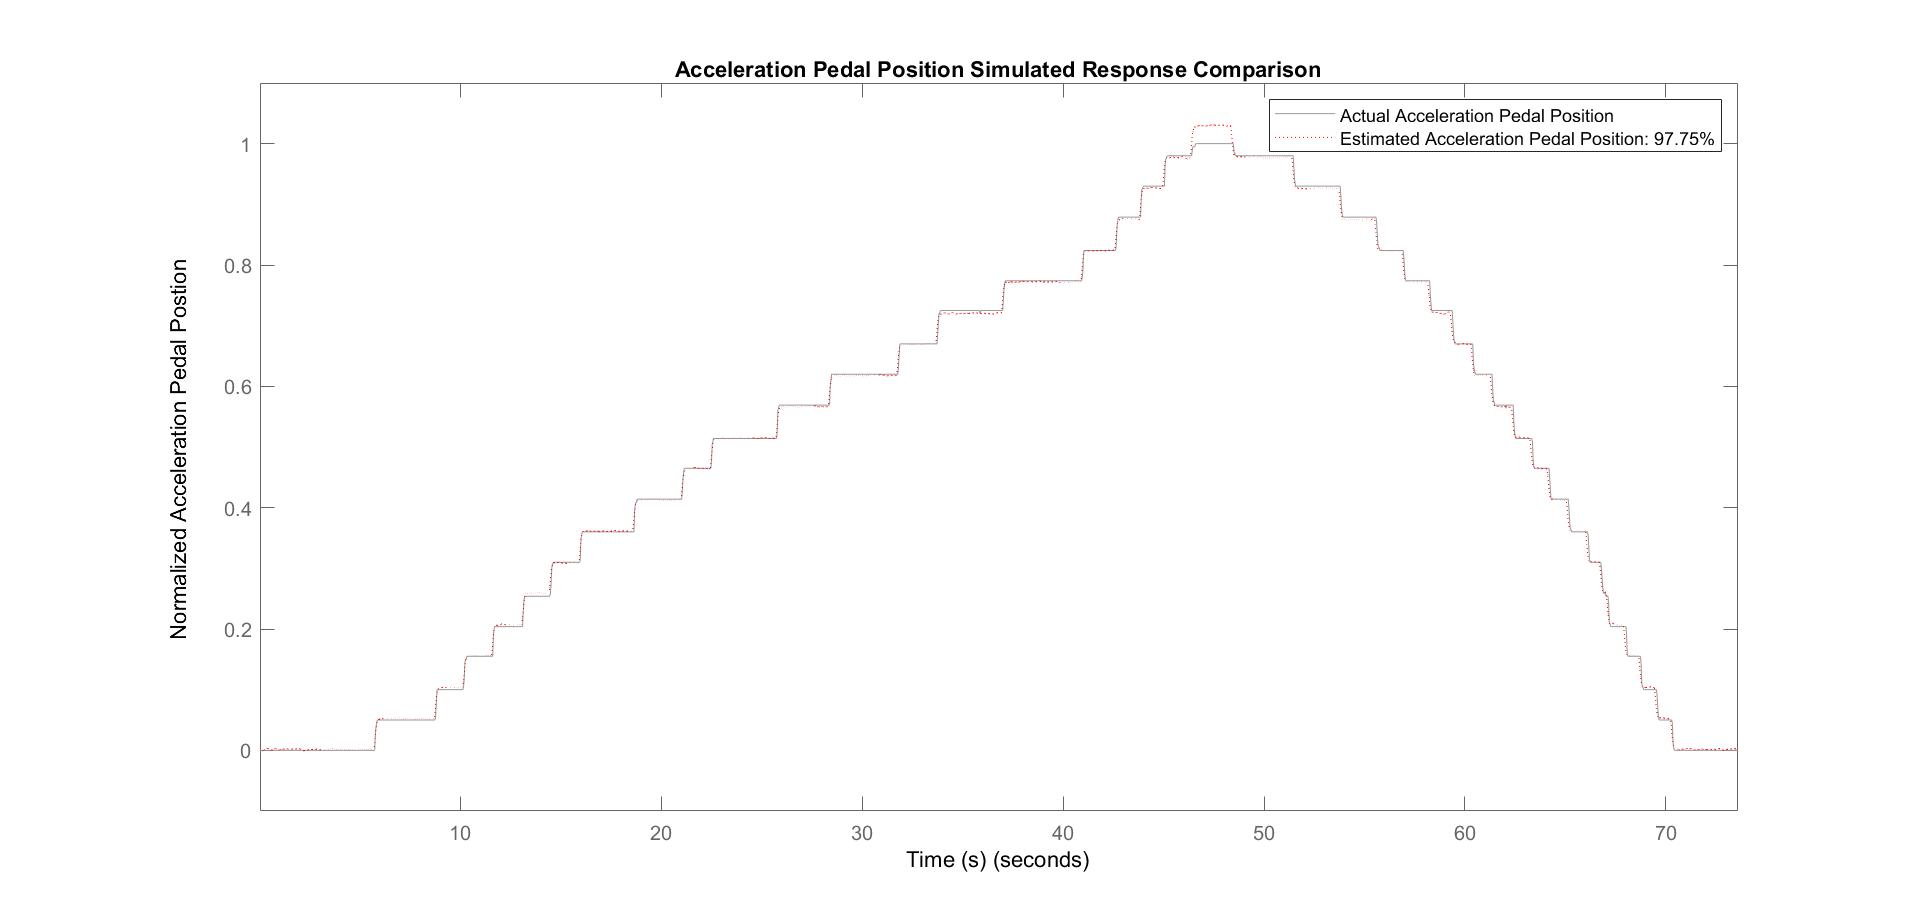
\includegraphics[width=0.48\linewidth]{figs/img/byWireAccelArxModel}}
	\subcaptionbox{Output of Estimated Manual System Model \label{manualAccelModel}}
		{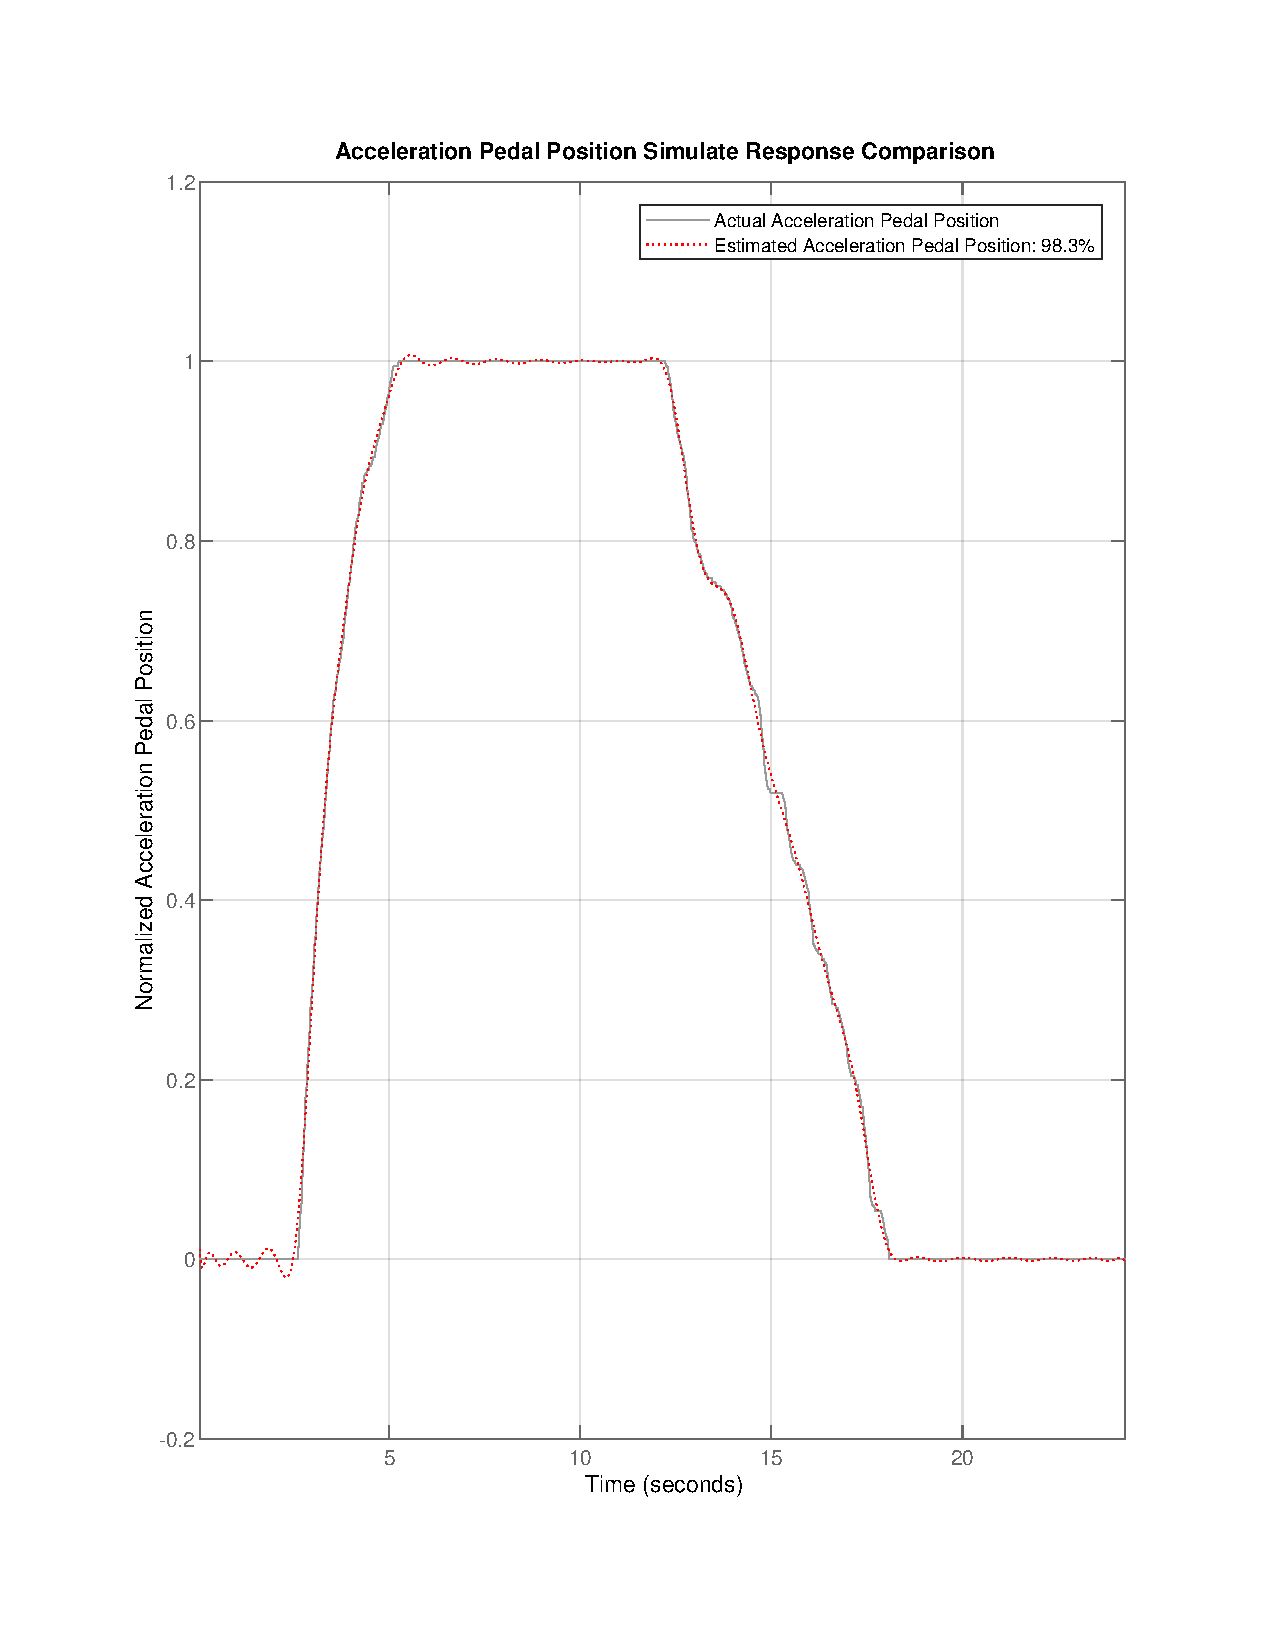
\includegraphics[width=0.48\linewidth]{figs/img/manualAccelTransferFunctionModel}}
	\caption{Acceleration System Estimated Pedal Position Comparison}
\end{figure}

\vspace{12pt}
\noindent The model of the by-wire acceleration system is a fourth order ARX model. The fourth order ARX model defined below represents the output acceleration pedal position, A(z), based on input torque voltage A, $B_1(z)$, and input torque voltage B, $B_2(z)$. 
% 
	\begin{align*}
		A(z)y(t) &= B_1(z)u_1(t) + B_2(z)u_2(t) + e(t),
	\end{align*}
	%
	where na = 4, nb = 4, nk = 0, and, 
	%
  \begin{align*}
		A(z) &= 1 - 1.018z^{-1} - 0.002901z^{-2} + 0.4631z^{-3} - 0.2038z^{-4}\\
    B_1(z) &= -0.0207 - 0.01912z^{-1} - 0.02159z^{-2} - 0.03307z^{-3}\\
		B_2(z) &= 0.02017 + 0.01833z^{-1} + 0.09461z^{-2} + 0.05683z^{-3}
  \end{align*}
%

\vspace{12pt}
\noindent The model of the manual acceleration system is a twenty-fourth order transfer function. The twenty-fourth order transfer function is the best proposed estimation considering the system costs associated with a higher order transfer function while also obtaining an acceptable best fit percentage. Table~\ref{tab:manualAccelCoeffA} shows the coefficients of the twenty-fourth order transfer function for the output acceleration pedal position with respect to the input torque voltage A signal. %
%
\begin{table}[hbtp]
	\caption{Manual Mode Acceleration Transfer Function Torque Voltage A Coefficient Table}
	\label{tab:manualAccelCoeffA}
  \centering
  \resizebox{\linewidth}{!}{% Resize table to fit within \linewidth horizontally
    \begin{tabular}{*{25}{c}}
      \toprule
      $a_0$& $a_1$&$a_2$&$a_3$&$a_4$&$a_5$&$a_6$&$a_7$&$a_8$&$a_9$&$a_{10}$&$a_{11}$&$a_{12}$&$a_{13}$&$a_{14}$&$a_{15}$&$a_{16}$&$a_{17}$&$a_{18}$ &$a_{19}$&$a_{20}$&$a_{21}$&$a_{22}$&$a_{23}$&$a_{24}$\\
      \midrule
      2.307E7 & 8.369E7 & 9.137E8 & 1.992E9 & 3.753E9 & 5.454E9 & 5.548E9 & 5.869E9 & 3.453E9 & 3.161E9 & 1.54E9 & 9.654E8 & 3.556E8 & 1.789E8 & 5.082E7 & 2.071E7 & 4.569E6 & 1.498E6 & 2.553E5 & 6.532E4 & 8443 & 1559 & 147.3 & 15.5 & 1\\
      \bottomrule
    \end{tabular}}
    \begin{center}
    		\resizebox{0.4\linewidth}{!}{% Resize table to fit within \linewidth horizontally
    \begin{tabular}{*{7}{c}}
      \toprule
      $b_0$& $b_1$&$b_2$&$b_3$&$b_4$&$b_5$&$b_6$\\
      \midrule
      -5.741E6 & -2.644E7 & -2.797E6 & -1.304E7 & -3.203E6 & -1.159E6 & -5.519E5\\
      \bottomrule
    \end{tabular}}
    \end{center}
\end{table}
%

\noindent Table~\ref{tab:manualAccelCoeffB} shows the coefficients of the twenty-fourth order transfer function for the output acceleration pedal position with respect to the input torque voltage B signal.%
%
\begin{table}[hbtp]
	\caption{Manual Mode Acceleration Transfer Function Torque Voltage B Coefficient Table}
	\label{tab:manualAccelCoeffB}
  \centering
  \resizebox{\linewidth}{!}{% Resize table to fit within \linewidth horizontally
    \begin{tabular}{*{25}{c}}
      \toprule
      $a_0$& $a_1$&$a_2$&$a_3$&$a_4$&$a_5$&$a_6$&$a_7$&$a_8$&$a_9$&$a_{10}$&$a_{11}$&$a_{12}$&$a_{13}$&$a_{14}$&$a_{15}$&$a_{16}$&$a_{17}$&$a_{18}$ &$a_{19}$&$a_{20}$&$a_{21}$&$a_{22}$&$a_{23}$&$a_{24}$\\
      \midrule
      5.224E6 & 4.205E7 & 1.429E8 & 3.233E8 & 5.444E8 & 7.326E8 & 8.247E8 & 7.402E8 & 6.301E8 & 3.99E8 & 2.731E8 & 1.264E8 & 7.223E7 & 2.48E7 & 1.216E7 & 3.084E6 & 1.324E6 & 2.422E5 & 9.264E4 & 1.159E4 & 4003 & 307.4 & 96.87 & 3.451 & 1\\
      \bottomrule
    \end{tabular}}
    \begin{center}
    	\resizebox{0.4\linewidth}{!}{% Resize table to fit within \linewidth horizontally
    \begin{tabular}{*{7}{c}}
      \toprule
      $b_0$& $b_1$&$b_2$&$b_3$&$b_4$&$b_5$&$b_6$\\
      \midrule
      -4.159E6 & 1.851E6 & -4.457E6 & 9.043E5 & -7.45E5 & 1.865E5 & -1.545E4\\
      \bottomrule
    \end{tabular}}
    \end{center}	
\end{table}
%
\subsubsection{Brake System}
While some by-wire models were created for the brake system, the models created using manual data were the only ones considered once we decided to use only manual data. It was found that a transfer function of 28 poles and 12 zeros gave an acceptable best fit percentage for most of the data log combinations that were tried. However, it was only within the 5\% error bound for one of the data log combinations. Another problem was that the brake system required four transfer functions, one for each input. Once these transfer functions were exported, there was uncertainty on how to connect them in order to produce the output value. As a result, we ended up switching to using Neural Networks to create a model for the brake system. 

\subsection{Neural Network Modeling}
\label{sec:NN-Modeling}

\subsubsection{Steering System}

To develop the model of the steering system using a neural network architecture, we used one data subset to train the model and then used an additional subset of data to verify the model worked. The neural network model used a feedforward network that had one hidden layer containing three neurons. The model was also trained with twelve delay units to achieve the required accuracy, meaning that the first twelve output samples of the model should be ignored.

\begin{figure}[htbp]
	\centering
	\subcaptionbox{Model Output Tracking and Error Plots for Data Subset 1 \label{initalBrakeModel}}
		{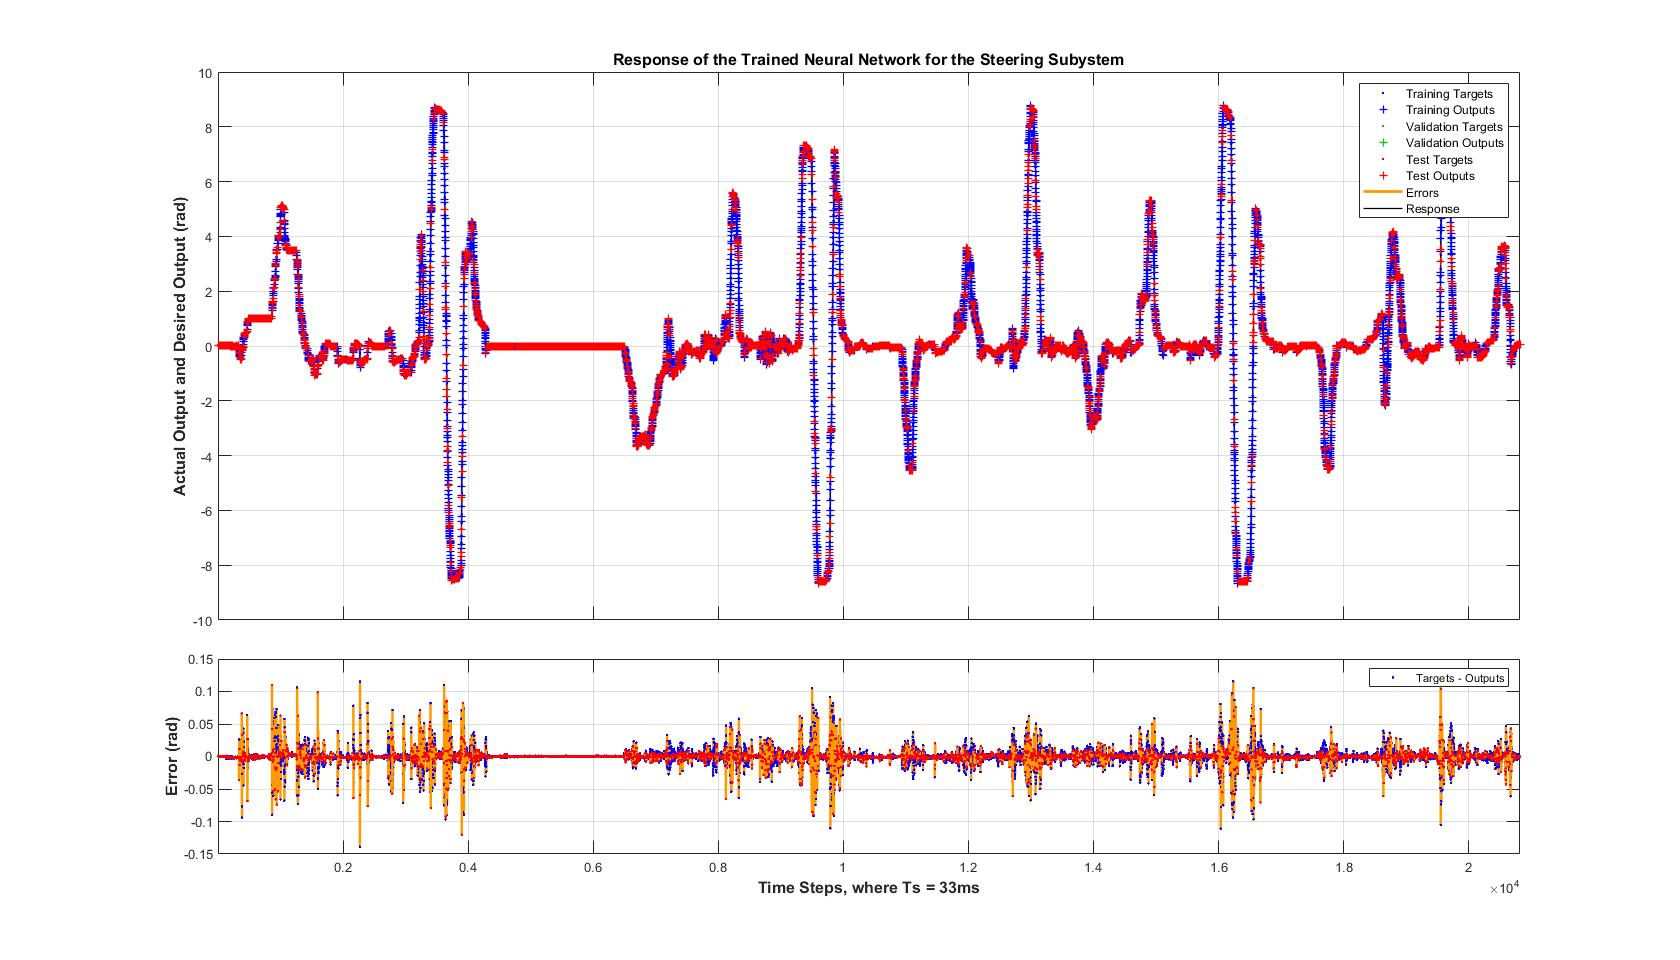
\includegraphics[width=0.48\linewidth]{figs/img/steeringNeuralNetworkTrainedOutput}}
	\subcaptionbox{Model Output Tracking and Error Plots for Data Subset 2 \label{testedBrakeModel}}
		{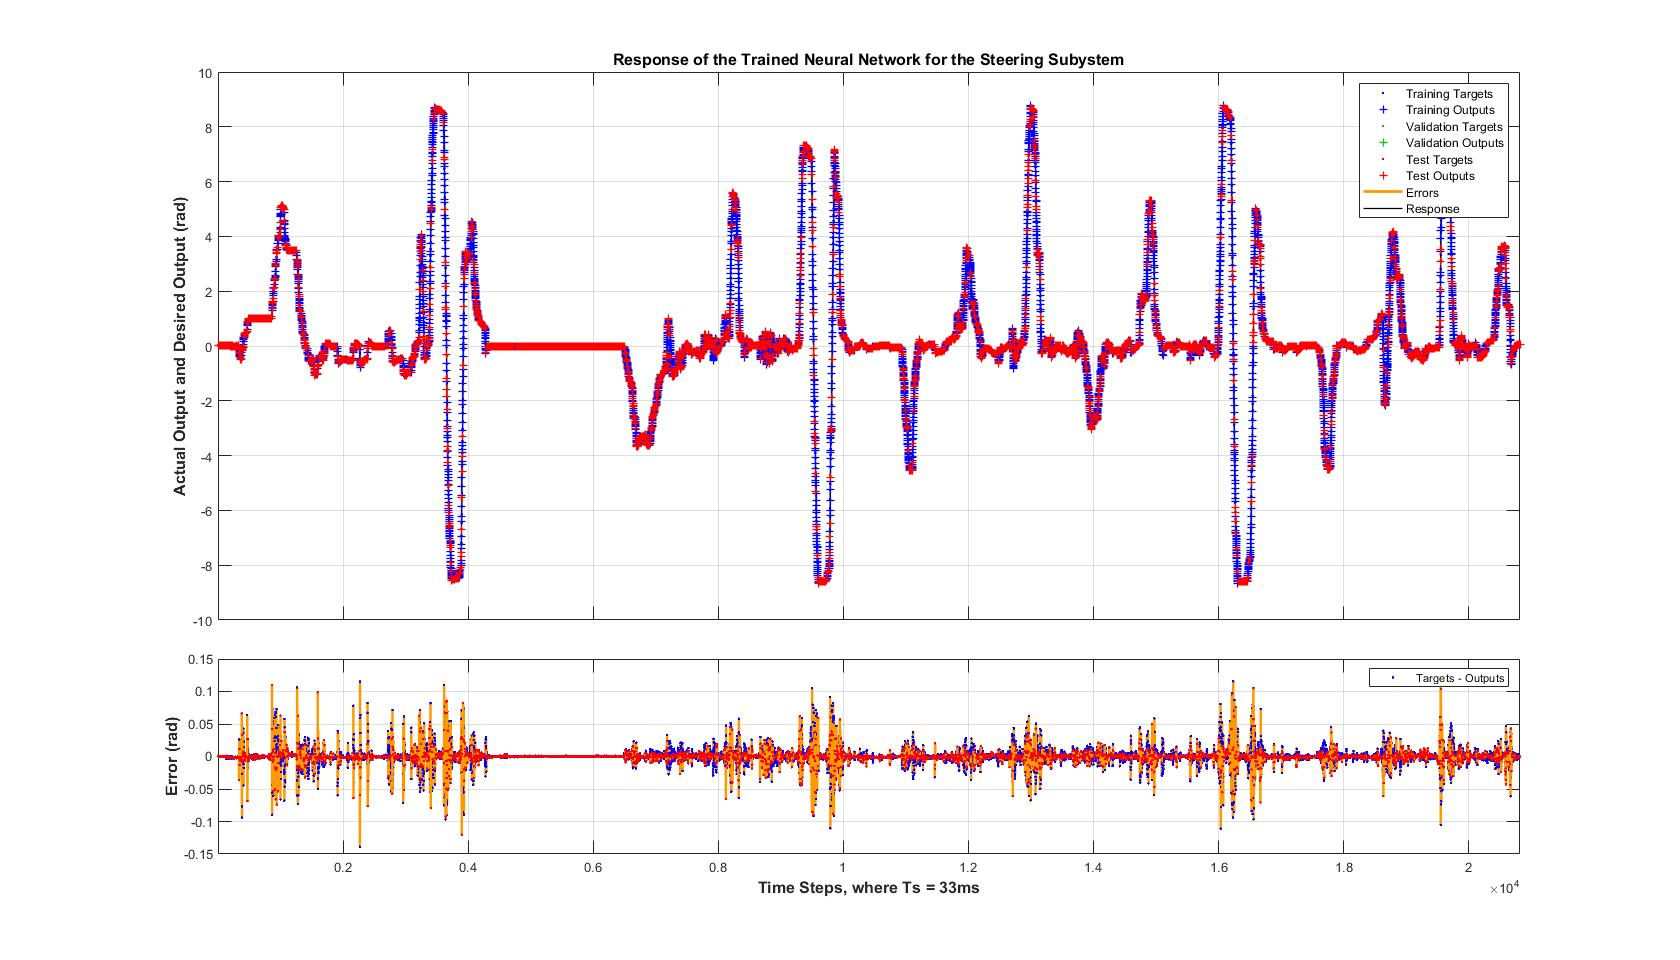
\includegraphics[width=0.48\linewidth]{figs/img/steeringNeuralNetworkTrainedOutput}}
	\caption{Steering System Training Plots}
\end{figure}


\subsubsection{Acceleration System}

To develop the model of the acceleration system using a neural network architecture, we used one data subset to train the model and then used an additional subset of data to verify the model worked. The neural network model used a feedforward network that had one hidden layer containing three neurons. The model was also trained with three delay units to achieve the required accuracy, meaning that the first three output samples of the model should be ignored. 

\begin{figure}[htbp]
	\centering
	\subcaptionbox{Model Output Tracking and Error Plots for Data Subset 1 \label{initalBrakeModel}}
		{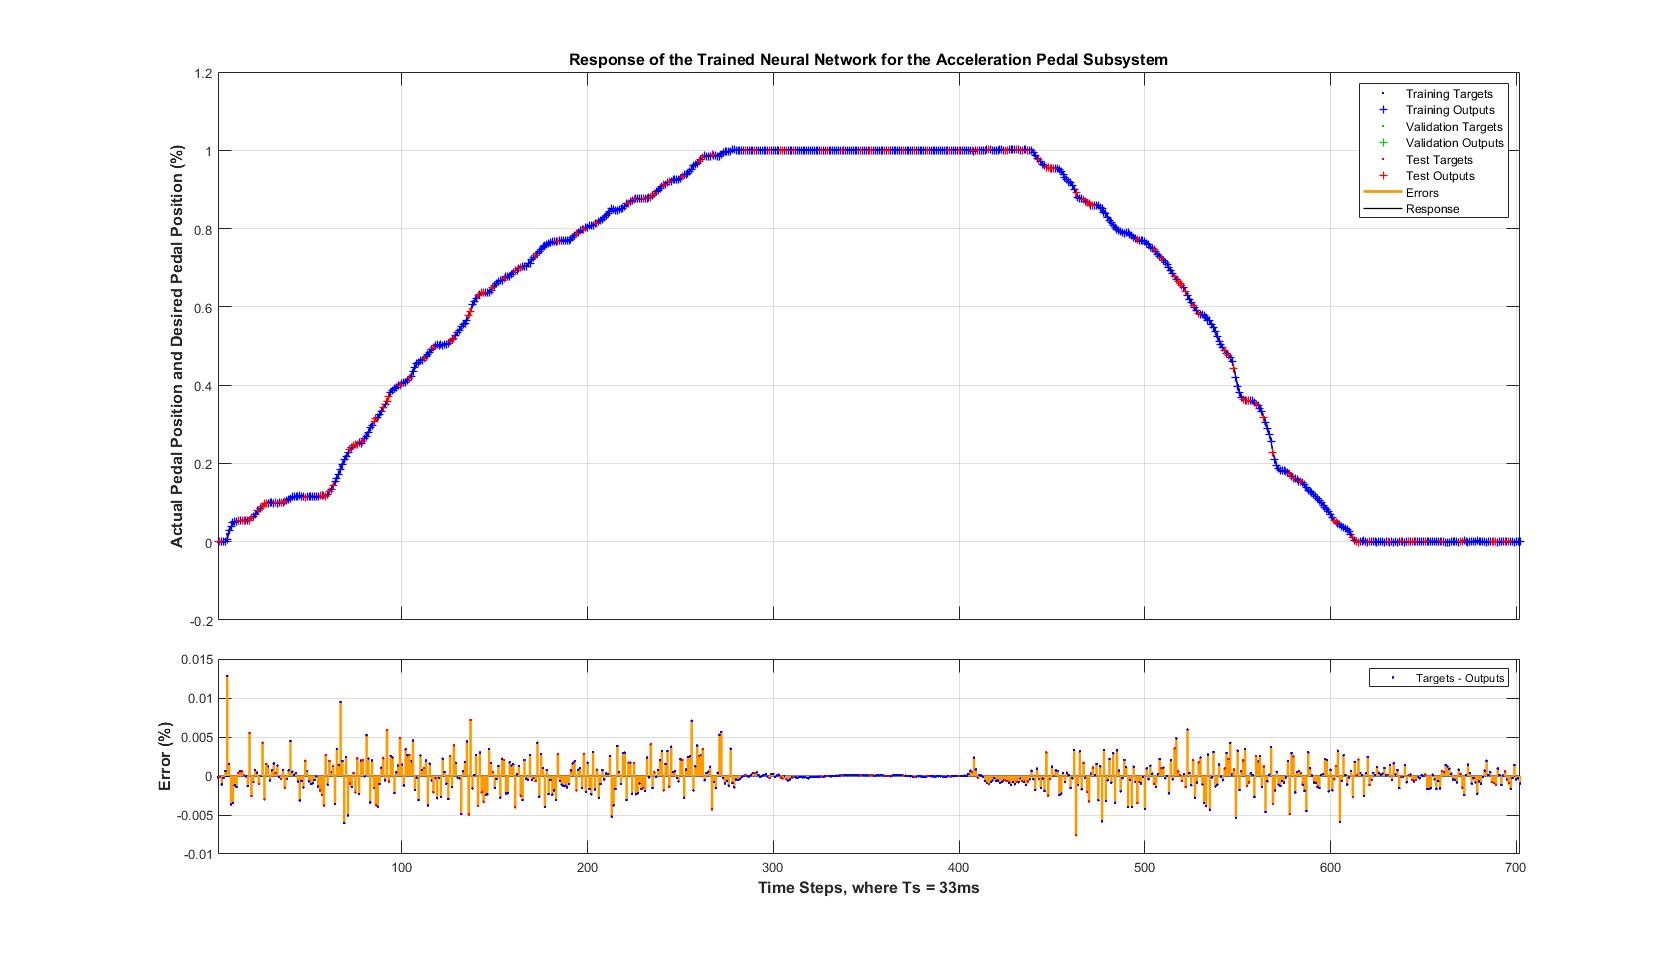
\includegraphics[width=0.48\linewidth]{figs/img/accelNeuralNetworkTrainedOutput}}
	\subcaptionbox{Model Output Tracking and Error Plots for Data Subset 2 \label{testedBrakeModel}}
		{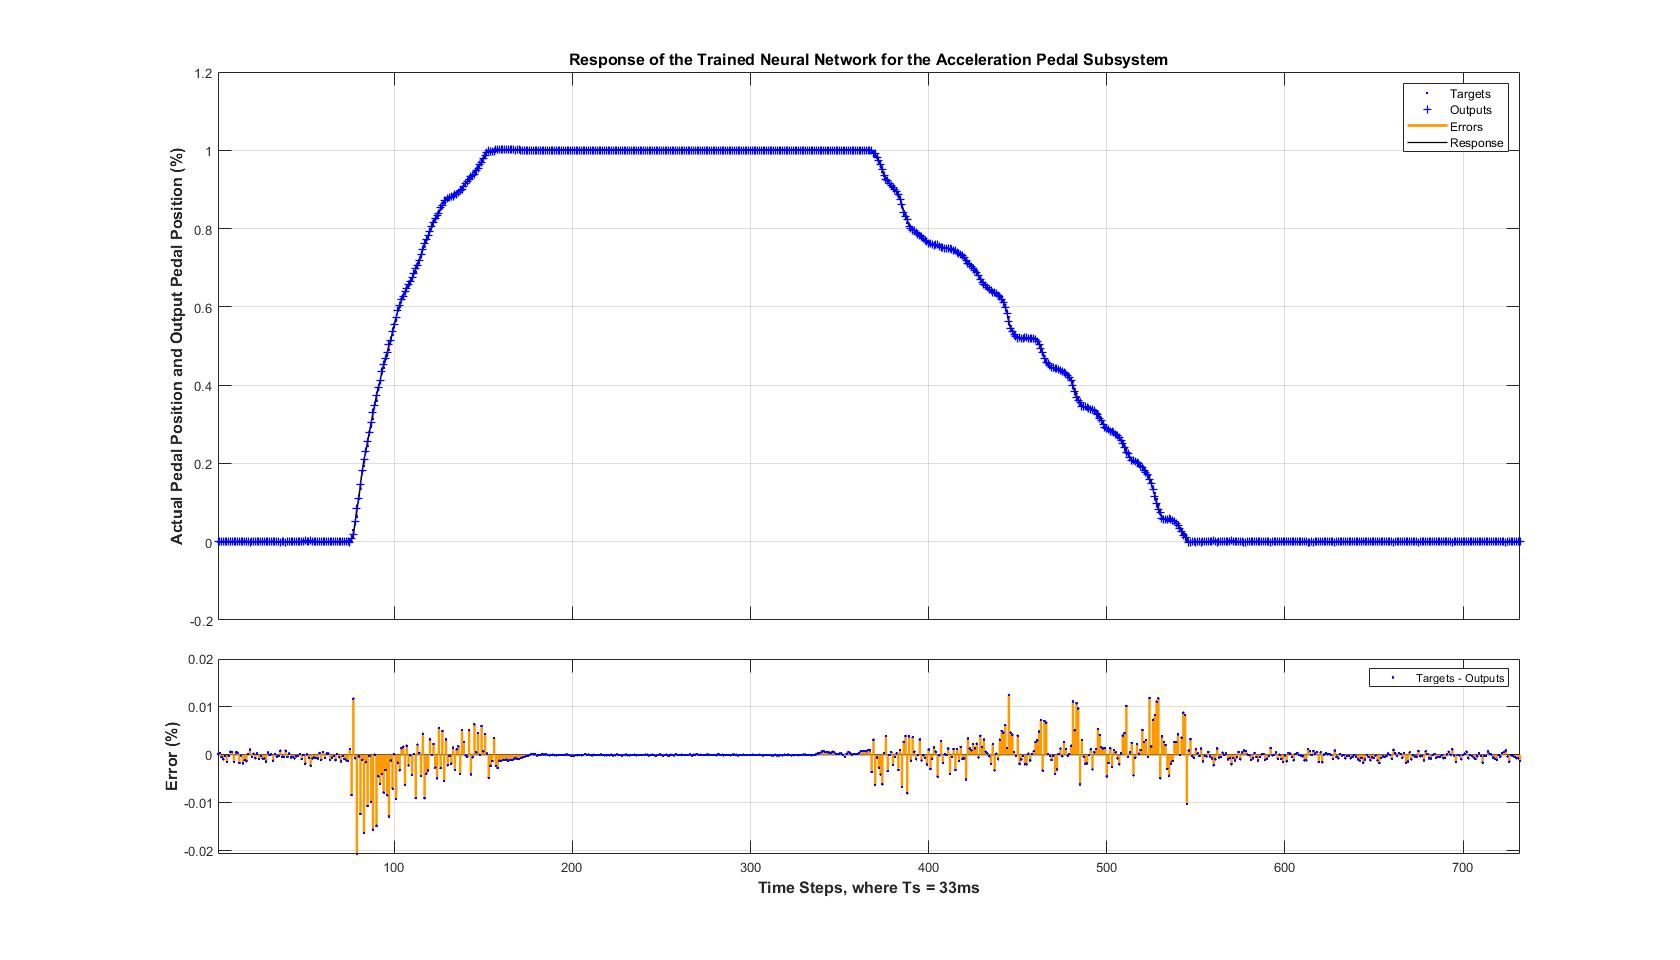
\includegraphics[width=0.48\linewidth]{figs/img/accelNeuralNetworkTrainedOutput2}}
	\caption{Acceleration System Training Plots}
\end{figure}


\subsubsection{Brake System}

The brake system was modeled using only the manual log data. It was trained using the data from the first brake log, and the result and error plots can be seen in \autoref{initalBrakeModel}. The plots show that the model is able to predict the outputs relatively accurately, along with keeping the error below 5\%. In order to further verify the accuracy of the model, it was tested using data from the second brake log. The results from that test, shown in \autoref{testedBrakeModel}, also show that the model can accurately predict the output values and do this within the accepted error bound of 5\%.
\begin{figure}[h]
	\centering
	\subcaptionbox{Model Output Tracking and Error Plots \label{initalBrakeModel}}
		{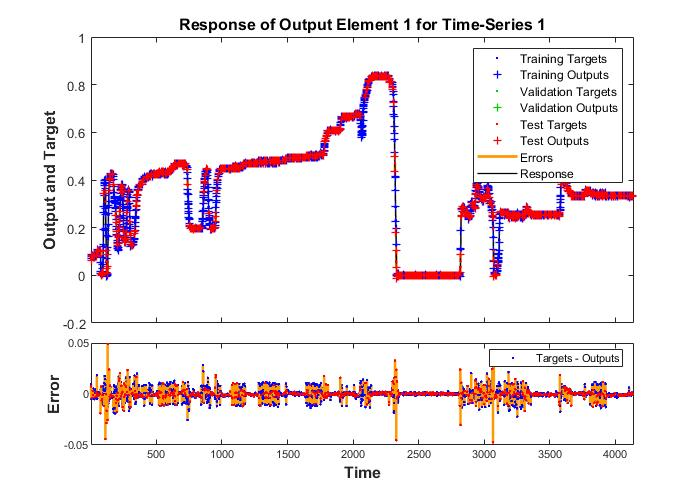
\includegraphics[width=0.48\linewidth]{figs/img/brake_new_neuralNetworkFig}}
	\subcaptionbox{Model Output Tracking and Error Plots for Log Two Data \label{testedBrakeModel}}
		{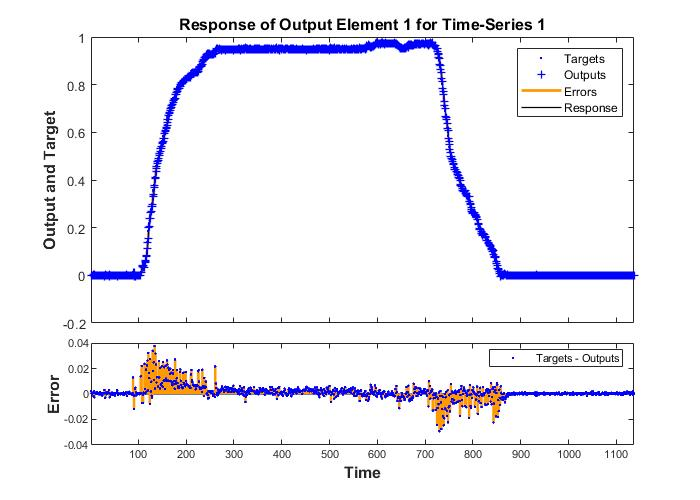
\includegraphics[width=0.48\linewidth]{figs/img/brake_new_neuralNetworkFigLog2Test}}
	\caption{Brake System Training Plots}
\end{figure}

Once the model was created, it was exported to Simulink and tested again. One test involved using To Workspace blocks to access the pressure voltages, position voltages, and desired pedal position values in the first brake log. These values were used as inputs for the model, and the actual pedal position along with the error between the desired and actual pedal positions were then plotted. The actual pedal position plot can be seen in \autoref{brakeWorkspacePedalPosition}. The resulting error plot between the desired pedal position and the model generated position can be found in \autoref{brakeWorkspacePedalError}. Despite an initial spike within the first few seconds of the graph, the error plot shows that the difference between the pedal positions generated by the system and the desired pedal positions is never more than 5\%. 

\begin{figure}[h]
	\centering
	\subcaptionbox{Actual Pedal Position \label{brakeWorkspacePedalPosition}}
		{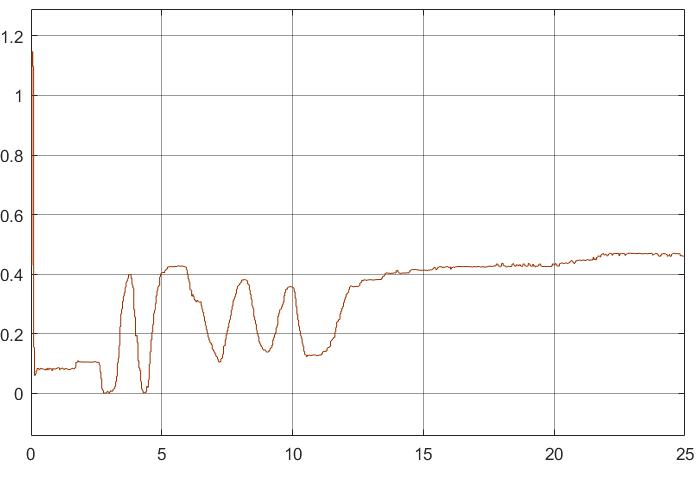
\includegraphics[width=0.48\linewidth]{figs/img/brakeSysActualPedalPositionFromWorkspaceBlocks}}
	\subcaptionbox{Error Between the Actual and Desired Pedal Position \label{brakeWorkspacePedalError}}
		{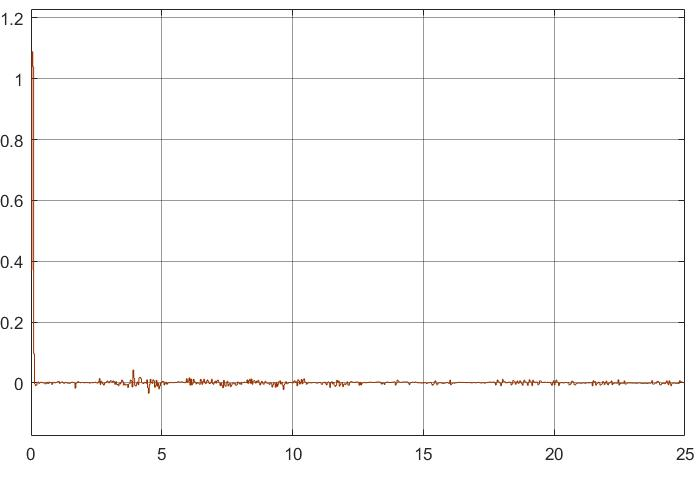
\includegraphics[width=0.48\linewidth]{figs/img/brakeSysPedalPositionErrorFromWorkspaceBlocks}}
	\caption{Actual Pedal Position and Error Plots Using the From Workspace Blocks}
\end{figure}


The second test used constant blocks to represent the voltages and desired pedal position at a specific time instant in the first brake log. The error and the actual pedal position were then plotted again. The pedal position plot is shown in \autoref{brakeConstantsPedalPosition}, and the error plot is represented by \autoref{brakeConstantsPedalError}. As the plots show, the model is able to produce the desired pedal position and the error falls to 0\% after a spike at the start. 

\begin{figure}[h]
	\centering
	\subcaptionbox{Actual Pedal Position \label{brakeConstantsPedalPosition}}
		{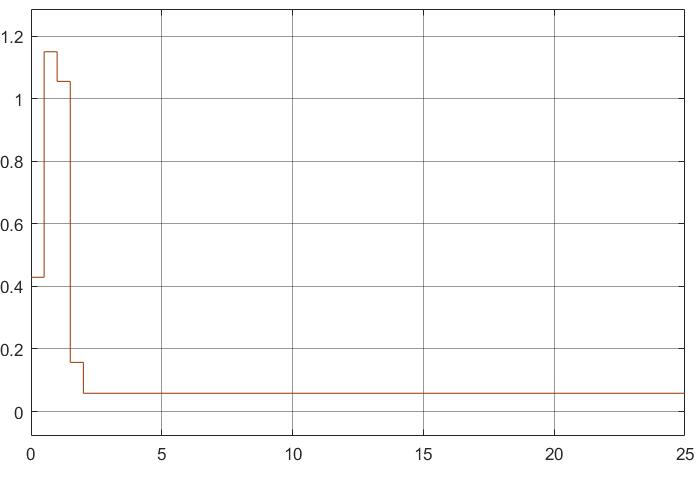
\includegraphics[width=0.48\linewidth]{figs/img/brakeSysActualPedalPositionConstantBlocks}}
	\subcaptionbox{Error Between the Actual and Desired Pedal Position \label{brakeConstantsPedalError}}
		{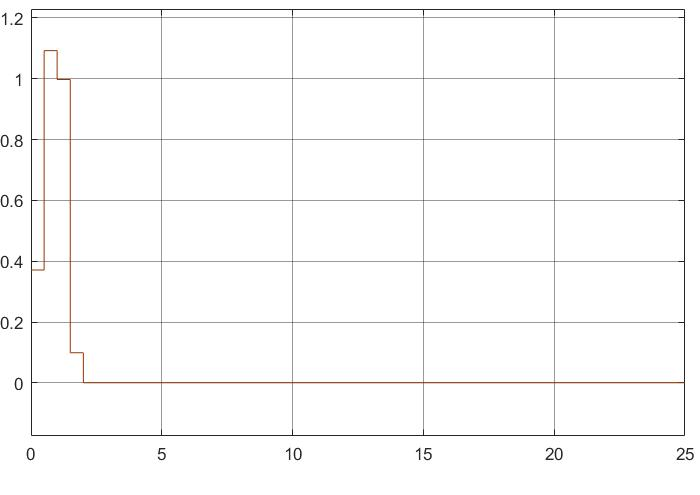
\includegraphics[width=0.48\linewidth]{figs/img/brakeSysPedalPositionErrorConstantBlocks}}
	\caption{Actual Pedal Position and Error Plots Using the Constant Blocks}
\end{figure}

\todo[inline]{Discuss results  NN modeling using the setup you explained in the previous section. See some IEEE papers}

\subsection{Discussion}
\label{sec:discussion}

For each vehicle subsystem, the results show that the neural network models were the most accurate models. Other models that we developed, such as the transfer function models, were relatively accurate when tracking the data, but those models were consistently falling outside of the error bounds that were defined at the start of the project. The neural network models, however, track the data more accurately and reduced the error significantly so that all error requirements were met. One downside to using neural networks as the plant model is it causes some complexities when trying to include these models into the HIL bench software for use in developing and testing controllers. 


\section{Conclusion and Future Work}
\label{sec:conclustionAndFutureWork}
Our initial approach was to model the subsystems using the System Identification Toolbox from MATLAB, but it produced unsatisfactory results. Switching to the Neural Network Time Series app allowed us to train models using the data we collected. These models that were developed met the predefined accuracy requirements, and so were tested using an open loop setup. In the future if AutonomouStuff would like to model other vehicle subsystems, we would recommend modeling them using Neural Networks. Creating the Neural Networks and exporting the models to Simulink was easy to do and produced accurate results. 

For this project, further testing should be completed for these subsystem models. Since time and availability constraints prevented us from testing the models using Hardware-in-the-Loop, this would be a good place to start. Further testing is important to make sure the developed models are accurate and compatible with testing using hardware. Depending on what AutonomouStuff decides, future engineers working on this project could start developing controllers based off of these models. Currently, AutonomouStuff develops their own controllers for their vehicle subsystems, but they could allow students to design some as part of this senior project. 

\section*{Acknowledgments}
The authors would like to thank Erik Guetz, Joe Buckner, Sai Chittemsetty, Matt Goben, and AutonomouStuff for their help and collaboration with this project. Without their support this project would never have been possible. 

\bibliographystyle{IEEEtran}
\bibliography{bib/references.bib}


% \begin{IEEEbiography}[{\includegraphics[width=1in,height=1.25in,clip,keepaspectratio]{a1.eps}}]{First A. Author} (M'76--SM'81--F'87) and all authors may include 
% biographies. Biographies are often not included in conference-related
% papers. This author became a Member (M) of IEEE in 1976, a Senior

%
% Member (SM) in 1981, and a Fellow (F) in 1987. The first paragraph may
% contain a place and/or date of birth (list place, then date). Next,
% the author's educational background is listed. The degrees should be
% listed with type of degree in what field, which institution, city,
% state, and country, and year the degree was earned. The author's major
% field of study should be lower-cased. 

% The second paragraph uses the pronoun of the person (he or she) and not the 
% author's last name. It lists military and work experience, including summer 
% and fellowship jobs. Job titles are capitalized. The current job must have a 
% location; previous positions may be listed 
% without one. Information concerning previous publications may be included. 
% Try not to list more than three books or published articles. The format for 
% listing publishers of a book within the biography is: title of book 
% (publisher name, year) similar to a reference. Current and previous research 
% interests end the paragraph. The third paragraph begins with the author's 
% title and last name (e.g., Dr.\ Smith, Prof.\ Jones, Mr.\ Kajor, Ms.\ Hunter). 
% List any memberships in professional societies other than the IEEE. Finally, 
% list any awards and work for IEEE committees and publications. If a 
% photograph is provided, it should be of good quality, and 
% professional-looking. Following are two examples of an author's biography.
% \end{IEEEbiography}

% \begin{IEEEbiography}[{\includegraphics[width=1in,height=1.25in,clip,keepaspectratio]{a2.eps}}]{Second B. Author} was born in Greenwich Village, New York, NY, USA in 
% 1977. He received the B.S. and M.S. degrees in aerospace engineering from 
% the University of Virginia, Charlottesville, in 2001 and the Ph.D. degree in 
% mechanical engineering from Drexel University, Philadelphia, PA, in 2008.

% From 2001 to 2004, he was a Research Assistant with the Princeton Plasma 
% Physics Laboratory. Since 2009, he has been an Assistant Professor with the 
% Mechanical Engineering Department, Texas A{\&}M University, College Station. 
% He is the author of three books, more than 150 articles, and more than 70 
% inventions. His research interests include high-pressure and high-density 
% nonthermal plasma discharge processes and applications, microscale plasma 
% discharges, discharges in liquids, spectroscopic diagnostics, plasma 
% propulsion, and innovation plasma applications. He is an Associate Editor of 
% the journal \emph{Earth, Moon, Planets}, and holds two patents. 

% Dr. Author was a recipient of the International Association of Geomagnetism 
% and Aeronomy Young Scientist Award for Excellence in 2008, and the IEEE 
% Electromagnetic Compatibility Society Best Symposium Paper Award in 2011. 
% \end{IEEEbiography}

% \begin{IEEEbiography}[{\includegraphics[width=1in,height=1.25in,clip,keepaspectratio]{a3.eps}}]{Third C. Author, Jr.} (M'87) received the B.S. degree in mechanical 
% engineering from National Chung Cheng University, Chiayi, Taiwan, in 2004 
% and the M.S. degree in mechanical engineering from National Tsing Hua 
% University, Hsinchu, Taiwan, in 2006. He is currently pursuing the Ph.D. 
% degree in mechanical engineering at Texas A{\&}M University, College 
% Station, TX, USA.

% From 2008 to 2009, he was a Research Assistant with the Institute of 
% Physics, Academia Sinica, Tapei, Taiwan. His research interest includes the 
% development of surface processing and biological/medical treatment 
% techniques using nonthermal atmospheric pressure plasmas, fundamental study 
% of plasma sources, and fabrication of micro- or nanostructured surfaces. 

% Mr. Author's awards and honors include the Frew Fellowship (Australian 
% Academy of Science), the I. I. Rabi Prize (APS), the European Frequency and 
% Time Forum Award, the Carl Zeiss Research Award, the William F. Meggers 
% Award and the Adolph Lomb Medal (OSA).
% \end{IEEEbiography}

\end{document}
